\documentclass[../main.tex]{subfiles}
\begin{document}
\chapter{Eigenvalues and Eigenvectors}
\section{Introduction}
\begin{theorem}[Fundemental Theorem of Algebra]
  \label{FTA}
  Let $p(z)$ be a polynomial of degree $m \geq 1$:
  \[
    p(z) = \sum_{j = 0}^{m}  c_jz^{j}
  \]
  where $c_j \in \C$, and $c_m \neq 0$.
  Then $p(z) = 0$ has exactly $m$ roots (not necessarily distinct) counted with multiplicity in $\C$.
\end{theorem}
\begin{definition}[Multiplicity]
  The root $z = w$ has \textit{multiplicity} $k$ if $(z - w)^{k}$ is a factor of $p(z)$ but $(z - w)^{k + 1}$ is not.
\end{definition}
\begin{definition}[Eigenvector and Eigenvalue]
  Let $T: V \to V$ be a linear map.
  Then $v \in V$ with $\vec{v} \neq 0$ is an \textit{eigenvector} of $T$ if:
  \[
    T(\vec{v}) = \lambda \vec{v}
  \]
  for a scalar $\lambda$ called the \textit{eigenvalue}.
\end{definition}
If $V = \R^{n} \text{ or } \C^{n}$, and $T$ is given in terms of an $n \times n$ matrix $A$, then:
\[
  A\vec{v} = \lambda \vec{v} \iff (A - \lambda I)\vec{v} = 0
\]
For a given $\lambda$, this holds for some vector $\vec{v} \neq 0$ if and only if $\det (A - \lambda I) = 0$.
This is because we require the kernel of $A - \lambda I$ to be nontrivial.

The equation obtained from this is called the \textit{characteristic equation}.
\begin{definition}[Characteristic Polynomial]
  For a matrix $A$, the \textit{characteristic polynomial} of degree $n$, $\chi_A$, is defined as:
  \[
    \chi_A(t) = \det (A - t I)
  \]
\end{definition}
From the definition of the determinant,
\begin{align*}
  \chi_A(t) &= \det (A - tI) \\
            &= \levi_{j_1 \ldots j_n}(A_{j_1 1} - t\delta_{j_1 1}) \cdots (A_{j_n n} - t\delta_{j_n n}) \\
            &= c_0 + c_1 t + \cdots + c_n t^{n}
\end{align*}
for some constants $c_0, \ldots, c_n$.

From this we can conclude the following:
\label{eigenvalueTrDet}
\begin{enumerate}
  \item $\chi_A(t)$ has degree $n$, and thus has $n$ roots.
    Hence, an $n \times n$ matrix has $n$ eigenvalues accounting for multiplicity.
  \item If $A$ is real, then all $c_i \in \R$, and thus eigenvalues are either real or come in conjugate pairs.
  \item
    $c_n = (-1)^{n}$ as we multiply $-t$ by itself $n$ times.
    Moreover:
    \[
      c_{n - 1} = (-1)^{n - 1}(A_{1 1} + \ldots + A_{n n}) = (-1)^{n - 1}\tr A
    \]
    We also know that $-\frac{c_{n - 1}}{c_n}$ is the sum of the roots, hence:
    \[
      t_1 + \cdots + t_n = -\frac{c_{n - 1}}{(-1)^n} = -\frac{(-1)^{n - 1}}{(-1)^{n}} = \tr A
    \]
    so the trace of a matrix is the sum of its eigenvalues.

    Finally,
    \[
      c_0 = \chi_A(0) = \det A
    \]
    We also know that $(-1)^{n} \frac{c_0}{c_n} = c_0$ is the product of the roots, hence:
    \[
      \det A = t_1 \cdots t_n
    \]
    so the determinant of a matrix is the product of its eigenvalues.
\end{enumerate}
\begin{example}
  \begin{enumerate}
    \item $V = \C^{2}$, $A = \begin{pmatrix}
        0 & -1 \\
        1 & 0 \\
        \end{pmatrix}$

      \textbf{Characteristic Polynomial}
      \[
        \chi_A(t) = \det (A - tI) = \det \begin{pmatrix}
        -t & -1 \\
        1 & -t \\
        \end{pmatrix} = t^2  + 1
      \]
      \textbf{Eigenvalues -} $\lambda = \pm i$.\par
      \textbf{Eigenvectors -}
      To get the eigenvector for $\lambda = i$:
      \[
        (A - iI)\vec{v} =
        \begin{pmatrix}
        -i & -1 \\
        1 & -i \\
        \end{pmatrix}
        \begin{pmatrix}
        x \\
        y \\
        \end{pmatrix} = \vec{0} \implies
        -ix - y = 0
      \]
      So the associated eigenvector is:
      \[
        \vec{v} = \alpha \begin{pmatrix}
        1 \\
        -i \\
        \end{pmatrix}
      \]
      for all $\alpha \in \C$.
      Similarly, for $\lambda = -i$, the associated eigenvector is  $\vec{v} = \alpha\begin{pmatrix}
      1 \\
      i \\
      \end{pmatrix}$ for all $\alpha \in \C$.
    \item $V = \R^2$, $A = \begin{pmatrix}
      1 & 1 \\
      0 & 1 \\
      \end{pmatrix}$

      \textbf{Characteristic Polynomial -} $\chi_A(t) = (t - 1)^2$.\par
      \textbf{Eigenvalues -} $\lambda  = 1$ with multiplicity 2.\par
      \textbf{Eigenvectors -} To get the eigenvector for $\lambda = 1$:
      \[
        (A - 1I)\vec{v} = \vec{0}  \iff \begin{pmatrix}
        0 & 1 \\
        0 & 0 \\
        \end{pmatrix}
        \begin{pmatrix}
        x \\
        y \\
        \end{pmatrix} = \vec{0} \implies y = 0
      \]
      So the associated eigenvector is $\vec{v} = \alpha \begin{pmatrix}
      1 \\
      0 \\
      \end{pmatrix}$ for all $\alpha \in \R$.
  \end{enumerate}
\end{example}
\section{Eigenspaces and Multiplicity}
\begin{definition}[Eigenspace]
  For an eigenvalue $\lambda$ of a matrix $A$, we define its \textit{eigenspace} by:
  \[
    E_\lambda = \{\vec{v} : A \vec{v} = \lambda \vec{v}\} = \ker (A - \lambda I)
  \]
  It is the collection of eigenvectors associated with a particular eigenvalue.
\end{definition}
\begin{definition}[Algebraic Multiplicity]
  The \textit{algebraic multiplicity}, denoted $M(\lambda)$ or $M_\lambda$, of an eigenvalue $\lambda$ is the multiplicity of $\lambda$ in the characteristic polynomial $\chi_A(t)$.
\end{definition}
By the fundamental theorem of algebra (\cref{FTA}), if $A$ is an $n \times n$ matrix, then the sum of all the algebraic multiplicities must be $n$. That is:
\[
  \sum_{\lambda} M(\lambda) = n
\]
\begin{definition}[Geometric Multiplicity]
  The \textit{geometric multiplicity}, denoted $m(\lambda)$ or $m_\lambda$, of an eigenvalue $\lambda$ is the dimension of its eigenspace:
  \[
    m_\lambda = \dim (E_\lambda)
  \]
\end{definition}
Equivalently, $m(\lambda)$ is the maximum number of linearly independent eigenvectors associated with the eigenvalue $\lambda$.
\begin{proposition}
  \label{multiplicityRelation}
  If $A$ is an $n \times n$ matrix with an eigenvalue $\lambda$, then $M_\lambda \geq m_\lambda$
\end{proposition}
\begin{proof}
  See \cref{multiplicityProof}.
\end{proof}
Note that this means if an eigenvalue as $M_\lambda = 1 \implies m_\lambda = 1$ since $m_\lambda > 0$.
\begin{definition}
  The \textit{defect}, denoted $\Delta_\lambda$ of an eigenvalue $\lambda$ is defined as:
  \[
    \Delta_\lambda = M_\lambda - m_\lambda
  \]
\end{definition}
By \cref{multiplicityRelation}, we have $\Delta_\lambda \geq 0$.
\begin{example}
  \begin{enumerate}
    \item Consider the matrix:\[
      A = \begin{pmatrix}
      4 & 1 & 0 \\
      0 & 4 & 1 \\
      0 & 0 & 4 \\
      \end{pmatrix}
    \]
    \textbf{Characteristic Polynomial -} $\chi_A(t) = (4 - t)^3$.\par
    \textbf{Eigenvalues -} $A$ only has one eigenvalue $\lambda = 4$ with $M_\lambda = 3$.\par
    \textbf{Eigenvectors}
    \[
      (A - 4\lambda)\vec{v} = \begin{pmatrix}
      0 & 1 & 0 \\
      0 & 0 & 1 \\
      0 & 0 & 0 \\
      \end{pmatrix}
      \begin{pmatrix}
      x \\
      y \\
      z \\
      \end{pmatrix} = \vec{0} \implies
      y = z = 0
    \]
    So the associated eigenvector is $\vec{v} = \alpha \begin{pmatrix}
    1 \\
    0 \\
    0 \\
    \end{pmatrix}$, thus $m_\lambda = 1$ as the eigenspace is:
    \[
      E_\lambda = \Span\left\{\begin{pmatrix}
      1 \\
      0 \\
      0 \\
      \end{pmatrix}\right\} \implies \dim (E_\lambda) = 1
    \]
    Therefore the defect is $\Delta_{\lambda} = 3 - 1 = 2$.
  \item Consider a reflection in the plane through $\vec{0}$ with normal $\vec{n}$.
    We do not need to use the matrix representation of this to compute the eigenvalues.
    Instead, we can use geometric intuition.

    Since $\vec{n}$ is just sent to $-\vec{n}$, that is, $H\vec{n} = -\vec{n}$, we have an eigenvector $\vec{n}$ with eigenvalue $\lambda = -1$.
    So $E_{-1} = \Span\{\vec{n}\}$

    Moreover, any vector $\vec{u}$ on the plane is unchanged, that is, $H \vec{u} = \vec{u}$ for all $\vec{u} \perp \vec{n}$.
    So we also have eigenvalue $\lambda = 1$ with $E_1 = \{\vec{x} : \vec{x} \cdot \vec{n} = \vec{0}\}$.

    Since $m_{-1} = 1$ and $m_1 = 2$ and $m_1 + m_2 \leq 3$, we must have all eigenvalues.
    Furthermore, since $M_\lambda \geq m_\lambda$, we must have $M_1 = 2$ and $M_{1} = 1$ so the geometric and algebraic multiplicities coincide for each eigenvalue.
  \item Consider a rotation $\Rot(\theta) \in \R^2$,
    \[
      \Rot(\theta) = \begin{pmatrix}
      \cos \theta & -\sin \theta \\
      \sin \theta & \cos \theta \\
      \end{pmatrix}
    \]
    \textbf{Characteristic Polynomial -} $\chi_{\Rot(\theta)}(t) = t^2 - 2t \cos \theta + 1$.\par
    \textbf{Eigenvalues -} It does not have real eigenvalues but does have eigenvalues in $\C$, $\lambda = e^{\pm i\theta}$.
    Note that this is a conjugate pair, as expected.\par
    \textbf{Eigenvectors -} The associated eigenvectors are:
    \[
      \vec{v} = \alpha \begin{pmatrix}
      1 \\
      \mp i \\
      \end{pmatrix}
    \]
    Since these both have $m_\lambda = 1$, they must also both have $M_\lambda = 1$.
  \item Consider a rotation by and $\theta$ about $\vec{n}$, $R(\theta, \vec{n})$.
    Note that:
    \[
      R(\theta, \vec{n})\vec{n} = \vec{n}
    \]
    So we have an eigenvalue $\lambda = 1$ with eigenspace $E_\lambda = \Span\{\vec{n}\}$.

    If we consider a basis given by $\vec{n}$ and two orthogonal vectors lying in the plane, $\vec{n}$ is unchanged under $R$ whereas the two vectors are rotated in the plane, similarity to as in \textbf{iii}.

    From \textbf{iii}, we know the rotation in the plane has eigenvalues $e^{\pm i \theta}$.
    Note that there are no other real eigenvalues unless $\theta = n\pi$, in which case, all vectors on the plane are eigenvectors with eigenvalue $\lambda = -1$ and algebraic multiplicity $M_{-1} = 2$ as both $e^{+i\pi}$ and $e^{-i\pi}$ coincide.

    So we have found all three complex eigenvalues.
  \item Consider the matrix
    \[
      A = \begin{pmatrix}
      -3 & -1 & 1 \\
      -1 & -3 & 1 \\
      -2 & -2 & 0 \\
      \end{pmatrix}
    \]
    \textbf{Characteristic Polynomial -} $\chi_A(t) = -(t + 2)^3$.\par
    \textbf{Eigenvalues -} $A$ only has eigenvalue $\lambda = -2$ with $M_\lambda = 3$.\par
    \textbf{Eigenvectors -} For the eigenvectors:
    \[
      (A + 2I) \vec{v} =
      \begin{pmatrix}
      -1 & -1 & 1 \\
      -1 & -1 & 1 \\
      -2 & -2 & 2 \\
      \end{pmatrix}
      \begin{pmatrix}
      x \\
      y \\
      z \\
      \end{pmatrix} = \vec{0}
    \]
    By eliminating $z$, we see that the general solution for this is:
    \[
      \begin{pmatrix}
      x \\
      y \\
      x + y \\
      \end{pmatrix} =
      x \begin{pmatrix}
      1 \\
      0 \\
      1 \\
      \end{pmatrix} + y\begin{pmatrix}
      0 \\
      1 \\
      1 \\
      \end{pmatrix}
    \]
    Therefore:
    \[
      E_\lambda = \Span\left\{\begin{pmatrix}
      1 \\
      0 \\
      1 \\
      \end{pmatrix},
      \begin{pmatrix}
      0 \\
      1 \\
      1 \\
      \end{pmatrix}\right\} \implies m_\lambda = 2
    \]
    So the eigenvalues do not form a basis of $\C^{3}$.
    The defect is $\Delta_\lambda = 3 - 2 = 1$.
  \end{enumerate}
\end{example}
\section{Diagonalisation and Similarity}
\begin{proposition}[Diagonalisble]
  \label{diagonalProp}
  If $A$ is a $n \times n$ matrix acting on $V = \R^{n}$ or $\C^{n}$, then the following statements are equivalent:
  \begin{itemize}
    \item There exists a basis of eigenvectors for $V$, $\{\vec{v}_1, \ldots, \vec{v}_n\}$ with $A \vec{v}_i = \lambda_i \vec{v}_i$.

      \textit{(Summation convention not used)}
    \item There exits an $n \times n$ invertible matrix $P$ with:
      \[
        P^{-1} A P = D = \begin{pmatrix}
        \lambda_1 &  &  \\
         & \ddots &  \\
         &  & \lambda_n \\
        \end{pmatrix}
      \]
      where $D$ is a \textit{diagonal matrix}, that is, all non-diagonal entries are $0$.
  \end{itemize}
  If either of these conditions is satisfied, $A$ is \textit{diagonalisable}.
\end{proposition}
\subsection{Linearly Independent Eigenvectors}
\begin{theorem}
  \label{linearlyIndependantEigenvectors}
  If an $n \times n$ matrix $A$ has distinct eigenvalues $\lambda_1, \ldots, \lambda_r$ with corresponding eigenvectors $\vec{v}_1, \ldots, \vec{v}_r$ then, $\{\vec{v}_1, \ldots, \vec{v}_r\}$ are linearly independent.
\end{theorem}
\begin{proof}
  Suppose, for contradiction, that $\{\vec{v}_1, \ldots, \vec{v}_r\}$ are linearly dependant.
  Then:
  \[
    \sum_{j = 1}^{r} \alpha_j \vec{v}_j = \vec{0}
  \]
  where not all $\alpha_j = 0$.

  There will be at least one such linear combination but we can take the minimal $p$ for which $\exists \alpha_1, \ldots, \alpha_p \neq 0$ with:
  \[
    \sum_{j = 1}^{p} \alpha_j \vec{v}_j = \vec{0}
  \]
  We are able to assume WLOG that this minimal linear combination occurs with the first $p$ vectors as we can just relabel the vectors.

  If we then apply the matrix $(A - \lambda_1 I)$, then we remove the first term of the sum, that is:
  \[
    (A - \lambda_1 I) \sum_{j = 1}^{p} \alpha_j \vec{v}_j = \sum_{j = 2}^{p} \alpha_j(\lambda_j - \lambda_1)\vec{v}_j
  \]
  Since $(A - \lambda_1 I)\vec{v}_1 = \vec{0}$.

  The above is a linear combination with $p - 1$ non-zero coefficients which contradicts the fact that $p$ was minimal.
  Thus $\{\vec{v}_1, \ldots, \vec{v}_r\}$ is linearly independent.
\end{proof}
\begin{remark}[Note]
  The above theorem and proof only hold when each eigenvalue has geometric multiplicity one, that is, each eigenvalue has exactly one associated eigenvector.
  However this does generalise to the following:

  Let $B_\lambda$ be a basis for the eigenspace $E_\lambda$ associated with $\lambda$.
  If $\lambda_1, \ldots, \lambda_r$ are distinct, then $B_{\lambda_1} \cup \cdots \cup B_{\lambda_r}$ is a linearly independent set.

  See \cref{gramSchmidt} for a construction of this in the case of Hermitian matrices.
\end{remark}
We can now prove \cref{diagonalProp}
\begin{proof}[\Cref{diagonalProp}]
  For any matrix $P$:
  \begin{itemize}
    \item $AP$ has columns $A\vec{C}_i(P)$.
    \item $PD$ has columns $\lambda_i\vec{C}_i(P)$ as $D$ is diagonal.
  \end{itemize}
  where $D$ is a diagonal matrix as in the proposition.
  So $AP = PD \iff A \vec{C}_i(P) = \lambda_i \vec{C}_i(P)\ \forall i = 1, \ldots, n$.

  \begin{proofdirection}{Suppose there exists a basis of eigenvectors for $V$}
    Given a basis of eigenvectors for $V$, the above relation allows us to determine such a $P$ as $\vec{C}_i(P)$ satisfies $A\vec{C}_i(P) = \lambda \vec{C}_i$ so we can take $\vec{C}_i(P) = \vec{v}_i$.

    Since we know what the eigenvectors form a basis for $V$, they are linearly independent and therefore the columns of $P$ are linearly independent so $\det P \neq 0$.
    Thus $P$ is invertible so we have constructed a $P$ such that $P^{-1} A P = D$.
  \end{proofdirection}
  \begin{proofdirection}{Suppose there exists such an invertible $P$}
    Since $P$ is invertible, $P^{-1} A P = D \iff AP = PD$.
    By the relation $A\vec{C}_i(P) = \lambda_i \vec{C}_i(P)$, we see that the columns of $P$ are eigenvectors.
    The columns of $P$ span $V$ so we have found a basis of eigenvectors for $V$.
  \end{proofdirection}
\end{proof}
\begin{remark}
  We see that the columns of $P$ are the eigenvectors of $A$.
  Since we need $P$ to be invertible, they must form a basis for $V$, which agrees with the equivalence of the two statements.
\end{remark}
\subsection{Criteria For Diagonalisability}
\subsubsection{A sufficient but not necessary condition}
\begin{proposition}
  If an $n \times n$ matrix has $n$ distinct eigenvalues, then it is diagonalisable.
\end{proposition}
\begin{proof}
If an $n \times n$ matrix has $n$ distinct eigenvalues, then by \cref{linearlyIndependantEigenvectors}, we have $n$ eigenvectors which are linearly independent.
This provides a basis of eigenvectors for $\R^{n}$ or $\C^{n}$.
So from \cref{diagonalProp}, $A$ is diagonalisable.
\end{proof}
Note that we require that all $n$ eigenvalues are distinct as otherwise we could have an eigenvalue with $m_\lambda < M_\lambda$ so would have less than $n$ linearly independent eigenvectors so would be unable to form a basis.
\subsubsection{A necessary and sufficient condition}
\begin{proposition}
  \label{diagonalisationIFF}
  $A$ is diagonalisable if and only if for all eigenvalues $\lambda$, $M_\lambda = m_\lambda$
\end{proposition}
\begin{proof}
  \begin{proofdirection}{Suppose $A$ is diagonalisable}
    Then by \cref{diagonalProp}, there exists a basis of $n$ eigenvectors for $V$.

    Suppose we have $m_{\lambda_i} < M_{\lambda_i}$ for some $\lambda_i$.
    Then since $m_\lambda \leq M_\lambda$ for all eigenvalues, $\sum_{\lambda} m_\lambda < \sum_{\lambda} M_\lambda = n$.

    However, this implies that $\sum_{\lambda} m_\lambda < n$ which contradicts the fact the eigenvectors form a basis for $V$.
    So we must have $m_\lambda = M_\lambda$ for all eigenvalues.
  \end{proofdirection}
  \begin{proofdirection}{Suppose $M_\lambda = m_\lambda$ for all $\lambda$}
    If $\lambda_i$ with $i = 1, \ldots, r$ are all the distinct eigenvalues of a matrix, then $B_{\lambda_1} \cup \cdots \cup B_{\lambda_r}$ is a linearly independent set, and its number of elements is:
    \[
      \sum_{i} m_{\lambda_i} = \sum_{i} M_{\lambda_i} = n
    \]
    so it must form a basis.
  \end{proofdirection}
\end{proof}
\subsection{Similarity}
\begin{definition}
  We say that two $n \times n$ matrices $A$ and $B$ are \textit{similar} if there exists an $n \times n$ invertible matrix $P$ such that:
  \[
    B = P^{-1}AP
  \]
\end{definition}
\begin{remark}
  Similar matrices represent the same linear map with respect to different bases.
  See \cref{COBSpecialCases}.
\end{remark}
\begin{proposition}
  \label{similarProperties}
  If $A$ and $B$ are similar, then:
  \begin{enumerate}
    \item $\det A = \det B$
    \item $\tr A= \tr B$
    \item $\chi_A(t) = \chi_B(t)$
  \end{enumerate}
\end{proposition}
\begin{proof}
  \begin{enumerate}
    \item Using $\det AB = \det A \det B$ and $\det P^{-1} = (\det P)^{-1}$, we see that:
      \[
        \det B = \det (P^{-1} A P) = \det (P^{-1}) \det (A) \det (P) = \det A
      \]
    \item Using $\tr(AB) = \tr(BA)$, we see that:
      \[
        \tr B = \tr(P^{-1} A P) = \tr(APP^{-1}) = \tr A
      \]
    \item Again, using $\det AB = \det A \det B$ and $\det P^{-1} = (\det P)^{-1}$, we see that:
      \begin{align*}
        \chi_B(t) &= \det(B - tI) \\
                  &= \det(P^{-1} A P - tI) \\
                  &= \det(P^{-1})\det(AP - tP) \\
                  &= \det(P^{-1})\det(A - tI)\det(P) \\
                  &= \det(A - tI) \\
                  &= \chi_A(t)
      \end{align*}
      So $\chi_A(t) = \chi_B(t)$, as required.
  \end{enumerate}
\end{proof}
\begin{remark}
  For the particular case of $B = D$ where $D$ is a diagonal matrix, this means that $A$ is diagonalisable.
  Utilising the fact that the determinant of a diagonal matrix is the product of the diagonal entries, we then have:
  \begin{enumerate}
    \item $\tr A = \sum_{i} \lambda_i$
    \item $\det A = \prod_{i} \lambda_i$
    \item $\chi_A(t) = (\lambda_1 - t) \cdots(\lambda_n - t)$
  \end{enumerate}
  These results are consistent with \cref{eigenvalueTrDet}.
\end{remark}
We can use these relations between similar matrices to provide a proof for \cref{multiplicityRelation}.
\begin{proof}
  \nonexaminable
  \label{multiplicityProof}
  Consider a basis for $E_\lambda$, $\{\vec{v}_1, \ldots, \vec{v}_r\}$ with $r = \dim E_\lambda = m_\lambda$.
  Using \cref{addBasis}, we can extend this to a basis for $V = \R^{n}$ or $\C^{n}$ by adding the vectors $\{\vec{w}_{r + 1}, \ldots, \vec{w}_n\}$.

  Define the $n \times n$ matrix P with columns such that:
  \begin{align*}
    \vec{C}_i(P) &= \vec{v}_i \text{ for } i = 1, \ldots, r \\
    \vec{C}_j(P) &= \vec{w}_i \text{ for } j = r + 1, \ldots, n \\
  \end{align*}
  Then, since $\vec{v}_i \in E_\lambda$ for $i = 1, \ldots, r$ we have:
  \[
    A \vec{C}_i = A \vec{v}_i = \lambda \vec{v}_i
  \]
  and for $\vec{C}_j$:
  \[
    A \vec{C}_j = A \vec{w}_j = \sum_{i} B_{i j}\vec{v}_i + \sum_{k} B_{k j}\vec{w}_k
  \]
  where $B$ is an $n \times n$ matrix with entries:
  \[
    B_{i j} = \begin{cases}
    \lambda \delta_{i j} & i, j = 1, \ldots, r \\
    0 & i = r + 1, \ldots, n \text{ and }j = 1, \ldots, r  \\
    \text{unknown} & i = 1, \ldots, n \text{ and }j = r + 1, \ldots, n
    \end{cases}
  \]
  We can rewrite with as $AP = PB$ and then, as $P$ is invertible since its columns form a basis for $V$, we have:
  \[
    P^{-1}AP = B =
      \left(\begin{array}{c|c}
      \lambda I & ? \\ \hline
      O & \hat{B}
      \end{array}\right)
  \]
  Where $?$ and $\hat{B}$ denote the unknown elements.
  From \cref{blockDeterminants}:
  \[
    \det(B - tI) = \det(\lambda I - tI)\det(\hat{B} - tI) = (\lambda - t)^{r}\det(\hat{B} - tI)
  \]
  From \cref{similarProperties}$, \chi_A(t) = \chi_B(t)$.
  Therefore:
  \[
    \chi_A(t)= (\lambda - t)^{r}\det(\hat{B} - tI)
  \]
  So the multiplicity of the root $\lambda$ must be at least $r$.
  Thus $M_\lambda \geq r = m_\lambda$.
\end{proof}
\subsection{Hermitian and Symmetric Matrices}
\begin{remark}[Recap] See \cref{transposeAndConjugate,complexInnerProduct} for further details.\par
  \textbf{Hermitian -} $A$ is Hermitian if and only if:
  \[
    A^{\dag} = \overline{(A^{\trans})} = A \iff A_{i j} = \overline{A_{j i}}
  \]
  \textbf{Symmetric -} $A$ is symmetric if and only if:
  \[
    A^{\trans} = A \iff A_{i j} = A_{j i}
  \]
  \textbf{Complex Inner Product -} For $\vec{v}, \vec{w} \in \C^{n}$:
  \[
    \vec{v}^{\dag}\vec{w} = \sum_{i} \overline{v_i}w_i
  \]
  \textbf{Real Inner Product - } For $\vec{v}, \vec{w} \in \R^{n}$, this reduces to:
  \[
    \vec{v}^{\trans}\vec{w} = \sum_{i} v_i w_i
  \]
\end{remark}
\begin{remark}
  If $A$ is hermitian, then:
  \[
    (A \vec{v})^{\dag}\vec{w} = \vec{v}^{\dag} A^{\dag} \vec{w} = \vec{v}^{\dag}(A\vec{w})
  \]
\end{remark}
\begin{theorem}
  \label{hermitianProperties}
  If $A$ is a $n \times n$ Hermitian matrix, then:
  \begin{enumerate}
    \item Every eigenvalue of $A$ is real.
    \item Eigenvectors $\vec{v}, \vec{w}$ with distinct eigenvalues, $\lambda, \mu$ are orthogonal, that is, $\vec{v}^{\dag} \vec{w} = 0$
    \item If $A$ is symmetric, then for any eigenvalues $\lambda$, we can construct a real eigenvector $\vec{v}$ so that \textbf{ii} reduces to  $\vec{v}^{\trans} \vec{w} = 0$
  \end{enumerate}
\end{theorem}
\begin{proof}
  \begin{enumerate}
    \item Consider an eigenvector $\vec{v}$ with eigenvalue $\lambda$, then:
    \begin{align*}
      \vec{v}^{\dag}(A \vec{v}) &= (A \vec{v})^{\dag}\vec{v} \\
      \vec{v}^{\dag}(\lambda \vec{v}) &=(\lambda \vec{v})^{\dag} \vec{v} \\
      \lambda \vec{v}^{\dag}\vec{v} &= \overline{\lambda}\vec{v}^{\dag}\vec{v}
    \end{align*}
    Since $\vec{v} \neq \vec{0}$, $\lambda = \overline{\lambda} \implies \lambda \in \R$.
  \item Consider eigenvectors $\vec{v}, \vec{w}$ with eigenvalues $\lambda, \mu$ respectively:
    \begin{align*}
      \vec{v}^{\dag}(A \vec{w}) &= (A \vec{v})^{\dag} \vec{w} \\
      \mu \vec{v}^{\dag}\vec{w} &= \overline{\lambda} \vec{v}^{\dag} \vec{w} \\
      \mu \vec{v}^{\dag}\vec{w} &= \lambda \vec{v}^{\dag} \vec{w}
    \end{align*}
    Since $\lambda \neq \mu$ we must have $\vec{v}^{\dag}\vec{w} = 0$, so $\vec{v}$ and $\vec{w}$ are orthogonal.
  \item Since $A$ is Hermitian and symmetric, $A$ must be real.
    From \textbf{i}, all eigenvalues must be real also.

    Consider an eigenvector $\vec{v} \in \C^{n}$ with eigenvalue $\lambda \in \R$.
    Let $\vec{v} = \vec{u} + i \vec{u}'$ with $\vec{u}, \vec{u}' \in \R^{n}$.
    Then:
    \begin{align*}
      A \vec{v} = \lambda \vec{v} \\
      A \vec{u} + i(A \vec{u}') = \lambda \vec{u} + i(\lambda \vec{u})
    \end{align*}
    Since $\lambda \in \R$, we must have:
    \[
      A \vec{u} = \lambda \vec{u} \text{ and } A \vec{u}' = \lambda \vec{u}'
    \]
    Furthermore, since $\vec{v} \neq \vec{0}$, at least one of $\vec{u}, \vec{u}' \neq \vec{0}$ so there is at least one real eigenvector.
  \end{enumerate}
\end{proof}
\subsection{Gram-Schmidt Orthogonalisation}
\label{gramSchmidt}
Given a linearly independent set of vectors in $\C^{n}$ $\{\vec{w}_1, \ldots, \vec{w}_r\}$.
Using the \textit{Gram-Schmidt Process}, we can construct a sequence of sets of the form:
\begin{center}
\begin{tabular}{c}
$\{\vec{w}_1, \vec{w}_2, \vec{w}_3, \ldots, \vec{w}_r\} $ \\
$\{\vec{u}_1, \vec{w}_2', \vec{w}_3', \ldots, \vec{w}_r'\} $ \\
$\{\vec{u}_1, \vec{u}_2, \vec{w}_3'', \ldots, \vec{w}_r''\} $ \\
$\vdots$ \\
$\{\vec{u}_1, \vec{u}_2, \vec{u}_3,\ldots, \vec{u}_r\} $ \\
\end{tabular}
\end{center}
where the final set, $\{\vec{u}_1, \vec{u}_2, \ldots, \vec{u}_n\}$, is an orthonormal set.

At each step of the process:
\begin{itemize}
  \item The span of the set is unmodified.
  \item The set is linearly independent.
  \item All of the $\vec{u}_i$ are orthonormal to each other.
  \item All of the $\vec{u}_i$ are orthogonal all of the $\vec{w}_i$.
\end{itemize}
\subsubsection{Construction}
\begin{itemize}
  \item \textbf{Step 1 -} Define $\vec{u}_1$ and $\vec{w}_j'$ for $j = 2, \ldots, r$ as:
    \[
      \vec{u}_1 = \frac{\vec{w}_1}{|\vec{w}_1|},\ \vec{w}_j' = \vec{w}_j  - (\vec{u}^{\dag}_{1}\vec{w}_j)\vec{u}_1
    \]
    This guarantees that $|\vec{u}_1| = 1$. We also see that:
    \begin{align*}
      \vec{u}^{\dag}_{1}\vec{w}_j' &= \vec{u}^{\dag}_{1}(\vec{w}_j - (\vec{u}^{\dag}_{1}\vec{w}_j)\vec{u}_1) \\
                                   &= \vec{u}^{\dag}_{1}\vec{w}_j - (\vec{u}^{\dag}_{1}\vec{w}_j)(\underbrace{\vec{u}^{\dag}_{1}\vec{u}_1}_{|\vec{u}_1| = 1}) \\
                                   &= \vec{u}^{\dag}_{1}\vec{w}_j -\vec{u}^{\dag}_{1}\vec{w}_j = 0
    \end{align*}
    So $\vec{u}^{\dag}_{1}\vec{w}_j' = 0$ for $j = 2, \ldots, r$.
  \item \textbf{Step 2 -} Define $\vec{u}_2$ and $\vec{w}_j''$ for $j = 3, \ldots, r$ as:
    \[
      \vec{u}_2 = \frac{\vec{w}_2'}{|\vec{w}_2|},\ \vec{w}_j'' = \vec{w}_j' - (\vec{u}^{\dag}_{2}\vec{w}_j')\vec{u}_2
    \]
    This guarantees that:
    \begin{itemize}
      \item $|\vec{u}_2| = 1$
      \item $\vec{u}_1$ and $\vec{u}_2$ are orthogonal since:
        \[
          \vec{u}^{\dag}_{1}\vec{u}_2 = \frac{\vec{u}^{\dag}_{1}\vec{w}_2'}{|\vec{w}_2|} = 0
        \]
        where $\vec{u}^{\dag}_{1}\vec{w}_2' = 0$ by the construction from the previous step.
      \item $\vec{u}_1$ is orthogonal to $\vec{w}_j''$ for $j = 3, \ldots, r$ since:
        \[
          \vec{u}^{\dag}_{1}\vec{w}_j'' = \underbrace{\vec{u}^{\dag}_{1}\vec{w}_j}_{=0} -(\vec{u}^{\dag}_{2}\vec{w}_j')(\underbrace{\vec{u}^{\dag}_{1}\vec{u}_2}_{=0}) =0
        \]
      \item $\vec{u}_2$ is orthogonal to $\vec{w}_j''$ for $j = 3, \ldots, r$ because $\vec{u}^{\dag}_{2}\vec{w}_j'' = 0$ by the same argument as in Step 1.
    \end{itemize}
  \item \textbf{Step ...}\par
    Repeatedly apply the same construction for $r$ steps total.
\end{itemize}
Since the construction at each step preserves the properties listed earlier, we will end up with an orthonormal set of vectors.

If we have a Hermitian matrix $A$, we can use this process to obtain an orthonormal basis $B_\lambda$ for each eigenspace $E_\lambda$.
Since we established that all the eigenvectors associated with different eigenvalues of a hermitian matrix are orthogonal, if $\lambda_1, \ldots, \lambda_r$ are distinct eigenvalues of $A$, then $B_{\lambda_1} \cup \cdots \cup B_{\lambda_r}$ is an orthonormal set.
\subsection{Unitary and Orthogonal Diagonalisation}
\begin{theorem}
  If $A$ is a $n \times n$ hermitian matrix, then $A$ is diagonalisable.
\end{theorem}
More specifically, if $A$ is hermitian, then all of the following equivalent statements hold:
\begin{enumerate}
  \item There exists a basis for $\C^{n}$ of eigenvectors $\vec{u}_1, \ldots, \vec{u}_n \in \C^{n}$ with $A \vec{u}_i = \lambda_i \vec{u}_i$.
  \item There exists a $n \times n$ invertible matrix $P$ with $P^{-1}AP = D$ where:
    \begin{itemize}
      \item $D$ is a diagonal matrix with $\lambda_1, \ldots, \lambda_n$ on the diagonal
      \item $C_i(P) = \vec{u}_i$, i.e., the columns of $P$ are the eigenvectors.
    \end{itemize}
\end{enumerate}
\begin{remark}
  In addition, the eigenvectors, $\vec{u}_i$ can be chosen to be orthonormal, that is:
  \[
    \vec{u}^{\dag}_{i}\vec{u}_j = \delta_{i j}
  \]
  Equivalently, the matrix $P$ can be chosen to be unitary, so that $P^{-1} = P^{\dag}$ and thus $P^{\dag} A P = D$.

  When working with real matrices, for a $n \times n$ real \textbf{symmetric} matrix $A$ ($A^{\trans} = A$), the eigenvectors can be taken to be $\vec{u}_1, \ldots, \vec{u}_n \in \R^{n}$ (see \cref{hermitianProperties}) and can be chosen so that:
  \[
    \vec{u}^{\trans}_{i} \vec{u}_j = \vec{u}_i \cdot \vec{u}_j= \delta_{i j}
  \]
  Equivalently, $P$ can be chosen to be orthogonal, so that $P^{-1} = P^{\trans}$ and thus $P^{\trans} A P = D$.
\end{remark}
\section{Change of Basis}
\label{changeOfBasis}
Consider the real or complex vector spaces $V$ and $W$ with $\dim V = n$ and $\dim W = m$.
Let $T: V \to W$ be a linear map and let $\{\vec{e}_1, \ldots, \vec{e}_n\}$ be a basis of $V$ and $\{\vec{f}_1, \ldots, \vec{f}_m\}$ be a basis of $W$ such that $T$ is represented by an $m \times n$ matrix $A$ with respect to these bases.

From \cref{matrixDef}, this means that:
\[
  T(\vec{e}_i) = \sum_{j} \vec{f}_j A_{j i}
\]
Now let $\{\vec{e}_1', \ldots, \vec{e}_n'\}$ be a new basis of $V$ and $\{\vec{f}_1', \ldots, \vec{f}_m'\}$ be a new basis of $W$.
$T$ is represented with respect to these new basis by a $m \times n$ matrix $B$.
Namely:
\[
  T(\vec{e}_i') = \sum_{j} \vec{f}_j' B_{j i}
\]
Suppose that the bases are related by:
\[
  \vec{e}_i' = \sum_{k} \vec{e}_k P_{k i} \text{ and } \vec{f}_j' = \sum_{l} \vec{f}_l Q_{l j}
\]
where $P$ is a $n \times n$ matrix and $Q$ is a $m \times m$ matrix, both of which are invertible.
\begin{proposition}[Change of Basis Formula]
  If $A, B, P, Q$ are defined as above, then:
  \[
    B = Q^{-1} A P
  \]
  This defines the \textit{change of basis formula} for matrices of linear maps.
  $P$ and $Q$ are called the \textit{change of basis matrices}.
\end{proposition}
\begin{proof}
  Consider the image of an element from the new basis for $V$, $\vec{e}_i'$, under $T$.

  We first use the definition of $P$ to yield:
  \begin{align*}
    T(\vec{e}_i') &= T\left(\sum_{k} \vec{e}_k P_{k i} \right) \text{ (by definition of $P$)} \\
                  &= \sum_{k} T(\vec{e}_k)P_{k i} \text{ (by linearity)} \\
                  &= \sum_{k, j} \vec{f}_j A_{j k} P_{k i}  \text{ (by definition of $A$)}
  \end{align*}
  Secondly, we use the definition of $B$:
  \begin{align*}
    T(\vec{e}_i') &= \sum_{j} \vec{f}_j' B_{j i} \text{ (by definition of $B$)}\\
                  &= \sum_{j, l} \vec{f}_l Q_{l j}B_{j i} \text{ (by definition of $Q$)}\\
                  &= \sum_{k, j} \vec{f}_j Q_{j k}B_{k i} \text{ (relabel $l \mapsto j$, $j \mapsto k$)}
  \end{align*}
  We can then compare the coefficients of $\vec{f}_j$ in each expression for $T(\vec{e}_i)$:
  \begin{align*}
    \sum_{k} A_{j k}P_{k i} &= \sum_{k} Q_{j k}B_{k i} \\
    (AP)_{j i} &= (QB)_{j i} \\
    \implies AP &= QB
  \end{align*}
  Since $P$ and $Q$ are invertible, the result follows.
\end{proof}
\begin{remark}
  \begin{enumerate}
    \item From the definition of $A$ which represents $T$ with respect to the original bases $\{\vec{e}_i\}$ and $\{\vec{f}_j\}$, we see that  that column $i$ of $A$ consists of the components of $T(\vec{e}_i)$ with respect to $\{\vec{f}_j\}$.

      Similarly, for the matrix $B$ which represents $T$ with respect to the new bases $\{\vec{e}_i'\}$ and $\{\vec{f}_j'\}$,  column $i$ of $B$ consists of the components of $T(\vec{e}_i')$ with respect to $\{\vec{f}_j'\}$.
    \item Column $i$ of $P$ consists of the components of $\vec{e}_i'$ with respect to the original basis $\{\vec{e}_i\}$.

      Similarly, column $i$ of $Q$ consists of the components of $\vec{f}_i'$ with respect to the original basis $\{\vec{f}_j\}$
    \item If instead of changing in the direction:
      \begin{align*}
        \{\vec{e}_i\} &\to \{\vec{e}_i'\} \\
        \{\vec{f}_j\} &\to \{\vec{f}_j'\}
      \end{align*}
      we instead change in the converse direction, then $P' = P^{-1}$ and $Q' = Q^{-1}$.
      The original bases can then be obtained with:
      \[
        \vec{e}_i = \sum_{k} \vec{e}_k' P_{k i}' \text{ and } \vec{f}_j = \sum_{l} \vec{f}_l' Q_{l j}'
      \]
  \end{enumerate}
\end{remark}
\begin{example}
  Consider $\dim V = n = 2$ and $\dim W = m = 3$.
  Suppose the image of the original basis is given by:
  \begin{align*}
    T(\vec{e}_1) &= \vec{f}_1  + 2\vec{f}_2 - \vec{f}_3 \\
    T(\vec{e}_2) &= -\vec{f}_1  + 2\vec{f}_2 + \vec{f}_3
  \end{align*}
  Then, from remark \textbf{i} above, $A$ is represented by:
  \[
    A = \begin{pmatrix}
    1 & -1 \\
    2 & 2 \\
    -1 & 1 \\
    \end{pmatrix}
  \]

  Now consider a new basis for $V$, $\{\vec{e}_1', \vec{e}_2'\}$ that is related to $\{\vec{e}_1, \vec{e}_2\}$ by:
  \[
    \vec{e}_1' = \vec{e}_1 - \vec{e}_2 \text{ and } \vec{e}_2' = \vec{e}_1 + \vec{e}_2
  \]
  so, by remark \textbf{ii} above, $P$ is:
  \[
    P = \begin{pmatrix}
    1 & 1 \\
    -1 & 1 \\
    \end{pmatrix}
  \]
  Now consider a new basis for $W$, $\{\vec{f}_1', \vec{f}_2', \vec{f}_3'\}$ that is related to $\{\vec{f}_1, \vec{f}_2, \vec{f}_3\}$ by:
  \begin{align*}
    \vec{f}_1' &= \vec{f}_1 - \vec{f}_3 \\
    \vec{f}_2' &= \vec{f}_2 \\
    \vec{f}_3' &= \vec{f}_1 + \vec{f}_3
  \end{align*}
  So, again by remark \textbf{ii}, $Q$ is:
  \[
    Q = \begin{pmatrix}
    1 & 0 & 1 \\
    0 & 1 & 0 \\
    -1 & 0 & 1 \\
    \end{pmatrix}
  \]
  From the change of basis formula, we then have:
  \[
    B = Q^{-1}AP = \begin{pmatrix}
    2 & 0 \\
    0 & 4 \\
    0 & 0 \\
    \end{pmatrix}
  \]
  Thus, by remark \textbf{i}, the images of the new basis vectors are:
  \[
    T(\vec{e}_1') = 2\vec{f}_1',\ T(\vec{e}_2') = 4\vec{f}_2'
  \]
  We can check our answer by ensuring that the images of the original basis match:
  \begin{align*}
    T(\vec{e}_1') &= T(\vec{e}_1) - T(\vec{e}_2) \\
                  &= \vec{f}_1 + 2\vec{f}_2 - \vec{f}_3 - (-\vec{f}_1 + 2\vec{f}_2 + \vec{f}_3)) \\
                  &= 2\vec{f}_1 -2 \vec{f}_3 \\
                  &= 2\vec{f}_1'
  \end{align*}
  and:
  \begin{align*}
    T(\vec{e}_2') &= T(\vec{e}_1) + T(\vec{e}_2) \\
                  &= \vec{f}_1 + 2\vec{f}_2 - \vec{f}_3 + (-\vec{f}_1 + 2\vec{f}_2 + \vec{f}_3)) \\
                  &= 4\vec{f}_2 \\
                  &= 4\vec{f}_2'
  \end{align*}
  which is consistent \tick
\end{example}
\begin{remark}[Special Cases]
  \label{COBSpecialCases}
  \begin{enumerate}
    \item If $V = W$ and both have the same bases, that is, $\vec{e}_i = \vec{f}_i$ and $\vec{e}_i' = \vec{f}_i'$, then $P = Q$ so the change of basis formula becomes:
      \[
        B = P^{-1} A P
      \]
      Therefore, matrices represent the same linear map $T: V \to V$ if and only if they are \textbf{similar}.
    \item Consider the case $V = W = \R^{n} \text{ or }\C^{n}$ both with the standard basis $\{\vec{e}_i\}$.

      If there exists a basis of eigenvectors of $T$, $\{\vec{v}_1, \ldots, \vec{v}_n\}$, then we can construct this to be the new basis $\{\vec{e}_i' = \vec{v}_i\}$ and define $B$ to be the matrix of $T$ with respect to this new basis.

      It then follows that:
      \[
        B = D
      \]
      where $D$ is a diagonal matrix with $\lambda_1, \ldots, \lambda_n$ on the diagonal where $T(\vec{v}_i) = \lambda_i \vec{v}_i$ and thus $D = P^{-1} A P$.
      By definition:
      \[
        \vec{v}_i  = \sum_{j} \vec{e}_j P_{j i}
      \]
      That is, the eigenvectors are the columns of $P$.
      Hence $P$ is both the change of basis matrix and also the matrix that diagonalises $A$.
  \end{enumerate}
\end{remark}
\subsection{Changes in Vector Components Under Change of Basis}
We can also arrive at the change of basis formula by considering vectors within the two vector spaces under both sets of bases.

Consider a real or complex vector space $V$ and $\vec{x} \in V$.
Assume that $\{\vec{e}_i\}$ and $\{\vec{e}_i'\}$ are two bases of $V$ related by $P$ where:
\[
  \vec{x} = x_i \vec{e}_i = x_i' \vec{e}_i'
\]
Since the bases are related by $P$, we have:
\[
  \vec{e}_j' = \sum_{i} \vec{e}_i P_{i j}
\]
Substituting this into the relation from $\vec{x}$, we have:
\[
  \vec{x} = x_i \vec{e}_i = x_j' \vec{e}_j' = x_j'(\vec{e}_i P_{i j}) = (P_{i j}x_j')\vec{e}_i
\]
As the basis vectors are linearly independent, we can compare coefficients to yield:
\[
  x_i = P_{i j}x_j'
\]
This is the relation between vector components with respect to different bases related by $P$.
In matrix form this can be written as:
\[
  \vec{x} = \begin{pmatrix}
  x_1 \\
  \vdots \\
  x_n \\
  \end{pmatrix}=
  \begin{pmatrix}
  P_{1 1} & \cdots & P_{1 n} \\
  \vdots & \ddots & \vdots \\
  P_{n 1} & \cdots & P_{n n} \\
  \end{pmatrix}
  \begin{pmatrix}
  x_1' \\
  \vdots \\
  x_n' \\
  \end{pmatrix}
  = P\vec{x}'
\]
Similarly, consider a vector space $W$ and $y \in W$.
Assume $\{\vec{f}_i\}$ and $\{\vec{f}_i'\}$ are two bases of $W$ related by $Q$ where:
\[
  \vec{y} = y_j \vec{f}_j = y_j'\vec{f}_j'
\]
Since the bases are related by $Q$, by a similar argument to above, we have:
\[
  y_i = Q_{i j}y_j' \text{ or equivalently } \vec{y} = Q\vec{y}'
\]
Now, if we consider the definition of a linear map $T: V \to W$ in terms of a matrix $A$ in the original basis and a matrix $B$ in the new basis, we have:
\[
  \vec{y} = T(\vec{x}) \iff \vec{y} = A\vec{x} \text{ and } \vec{y}' = B\vec{x}'
\]
Therefore,
\[
  B\vec{x}' = \vec{y}' = Q^{-1} \vec{y} = Q^{-1}A \vec{x} = (Q^{-1} A P)\vec{x}'
\]
Thus $B = Q^{-1} A P$.
\section{Cayley-Hamilton Theorem}
\begin{theorem}[Cayley-Hamilton Theorem]
  If $A$ is an $n \times n$ matrix with:
  \[
    \chi_A(t) = \det(A - tI) = \sum_{r = 0}^{n} c_r t^{r}
  \]
  then,
  \[
    \chi_A(A) = \sum_{r = 0}^{n} c_r A^{r} = O
  \]
  That is, a matrix satisfies its own characteristic polynomial.
\end{theorem}
We will cover multiple different proofs of varying complexity for different types of matrices.
\begin{proof}[For $2 \times 2$ Matrices]
  We can write a general $2 \times 2$ matrix as:
  \[
    A = \begin{pmatrix}
    A_{1 1} & A_{1 2} \\
    A_{2 1} & A_{2 2} \\
    \end{pmatrix}
  \]
  Then:
  \begin{align*}
    \chi_A(t) &= t^2 - (\tr A)t + \det A \\
              &= t^2 - (A_{1 1} + A_{2 2})t + (A_{1 1}A_{2 2} - A_{1 2}A_{2 2})
  \end{align*}
  Then by substitution of $A$ into $\chi_A(t)$ we see that $\chi_A(A) = O$.
\end{proof}
\begin{proof}[Diagonalisible $n \times n$ Matrices]
  Consider an $n \times n$ matrix $A$ with eigenvalues $\lambda_i$ and invertible matrix $P$ such that:
  \[
    P^{-1} A P = D
  \]
  where $D$ is a diagonal matrix with $\lambda_i$ on the diagonal.
  Note that $D^{r}$ is also diagonal with:
  \[
    D^{r} = \begin{pmatrix}
    \lambda^{r}_{1} &  & \\
     & \ddots &  \\
     &  & \lambda^{r}_{n} \\
    \end{pmatrix}
  \]
  We can then substitute $D$ into $\chi_A$ and use the above to get the following:
  \[
    \chi_A(D) = \begin{pmatrix}
      \chi_A(\lambda_1) &  &  \\
                        & \ddots &  \\
                        &  & \chi_A(\lambda_n) \\
    \end{pmatrix} = O
  \]
  But $A = PDP^{-1}$ so $A^{r} = (PDP^{-1})^{r} = PD^{r}P^{-1}$.
  So when substituting $A$ into $\chi_A$ we can pull out $P$ and $P^{-1}$.
  Hence:
  \begin{align*}
    \chi_A(A) &= \chi(PDP^{-1}) \\
              &= P\chi_A(D)P^{-1} \\
              &= O
  \end{align*}
\end{proof}
\begin{proof}[General $n \times n$ Matrix]
  \nonexaminable
  Let $M = A- tI$, then
  \[
    \chi_A(t) = \det M = \sum_{r = 0}^{n} c_r t^{r}
  \]
  Recall that $\adj M =\widetilde{M}$, which satisfies:
  \[
    \widetilde{M}M = (\det M)I
  \]
  From \cref{adjugateDef}, we see that every entry of $\widetilde{M}$ is a cofactor of $M$.
  Therefore, each entry will be a polynomial in $t$ of degree at most $n - 1$.
  We can then define the matrices $B_r$ such that:
  \[
    \widetilde{M} = \sum_{r = 0}^{n - 1}  B_r t^{r}
  \]
  Therefore we can write $\widetilde{M} M$ as:
  \begin{align*}
    \widetilde{M} M &= \left(\sum_{r = 0}^{n - 1} B_r t^{r}\right)(A - tI) \\
                    &= B_0 A - (B_1 A - B_0)t + (B_2 A - B_1)t^2 + \cdots \\
                    &\quad + (B_{n - 1}A - B_{n- 2})t^{n - 1} - B_{n - 1}t^{n}
  \end{align*}
  Comparing coefficients of $t$ in $\widetilde{M} M$ and $(\det M)I$, we have:
  \begin{align*}
    c_0 I &= B_0 A \\
    c_1 I &= B_1 A - B_0 \\
    c_2 I &= B_2 A - B_1 \\
          &\ \ \vdots \\
    c_{n-1}I &= B_{n - 1}A - B_{n - 2} \\
    c_n I &= -B_{n - 1}
  \end{align*}
  If we multiply both sides by ascending powers of $A$, we get the terms of $\chi_A(A)$ on the left hand side:
  \begin{align*}
    c_0 I &= B_0 A \\
    c_1 A &= B_1 A^2 - B_0A \\
    c_2 A^2 &= B_2 A^3 - B_1A^2 \\
          &\ \ \vdots \\
    c_{n-1}A^{n - 1} &= B_{n - 1}A^{n} - B_{n - 2}A^{n - 1} \\
    c_n A^{n} &= -B_{n - 1}A^{n}
  \end{align*}
  The sum of the terms on the right hand side telescopes as follows:
  \[
    B_0A+B_1A^2 - B_0A + B_2 A^3 - B_1A^2 + \cdots + B_{n-1}A^{n} - B_{n-2}A^{n-1} -B_{n-1}A^{n} =O
  \]
  The sum of the terms on the left hand side is:
  \[
    \chi_A(A) = c_0 I + c_1 A + c_2 A^2 + \cdots c_{n - 1}A^{n - 1} + c_n A^{n}
  \]
  Thus $\chi_A(A) = O$.
\end{proof}
\section{Quadratic Forms}
\begin{definition}[Quadratic Form]
  A \textit{quadratic form} is a function $\mathcal{F}: \R^{n} \to \R$.
  \[
    \mathcal{F}(\vec{x}) = \vec{x}^{\trans}A\vec{x} = x_i A_{i j} x_j
  \]
  where $A$ is a real symmetric matrix.
\end{definition}
Since $A$ is a real symmetric matrix it can be diagonalised as:
\[
  P^{\trans} A P = D = \begin{pmatrix}
  \lambda_1 &  &  \\
   & \ddots &  \\
   &  & \lambda_n \\
  \end{pmatrix}
\]
where $\lambda_i$ are real eigenvalues and $P$ is a real orthogonal $n \times n$ matrix with orthonormal eigenvectors $\vec{u}_i$ as its columns.

If we set $\vec{x}' = P^{\trans} \vec{x} \iff \vec{x} = P\vec{x}'$, we can diagonalise $\mathcal{F}$.
Noting that $\vec{x}^{\trans} = (\vec{x}')^{\trans}P^{\trans}$, we have:
\[
  \mathcal{F}(\vec{x}) = \vec{x}^{\trans}A\vec{x} = (\vec{x}')^{\trans} P^{\trans} A \vec{x} = (\vec{x}')^{\trans}P^{\trans}AP\vec{x}' = (\vec{x}')^{\trans}D\vec{x}'
\]
Since $D$ is diagonal, we can easily compute this in terms of the components of $\vec{x}'$:
\begin{equation}
  \label{quadraticFormSum}
  \mathcal{F}(\vec{x}) = (\vec{x}')^{\trans}D \vec{x}' = \sum_{i}\lambda_i (x_i')^2
\end{equation}
We can write $\vec{x}'$ and $\vec{x}$ in the standard basis as:
\begin{align*}
  \vec{x}' &= x_1' \vec{e}_1 + \cdots + x_n' \vec{e}_n \\
  \vec{x} &= x_1 \vec{e}_1 + \cdots + x_n \vec{e}_n
\end{align*}
As $\vec{x} = P\vec{x}'$ and the columns of $P$ are the orthonormal eigenvectors $\vec{u}_i$ we can also write $\vec{x}$ as:
\begin{align*}
  \vec{x} &= x'_1(P\vec{e}_1) + \cdots + x_n'(P\vec{e}_n)\\
          &= x_1' \vec{u}_1 + \cdots + x_n'\vec{u}_n
\end{align*}
We can then take the dot product of this with $\vec{u}_i$ to extract the $i$-th component:
\[
  x_i' = \vec{x} \cdot \vec{u}_i
\]
So $x_i'$ are the components of $\vec{x}$ with respect to the new orthonormal basis vectors $\vec{u}_i$. We call the new axes along the these directions the \textit{principal axes} of $\mathcal{F}$.

Since these are related to the standard axes by the orthogonal matrix $P$, from \cref{orthogonalMatrices}, we see that:
\[
  |\vec{x}|^2 = x_i x_i = x_i'x_i'
\]
so the norm of $\vec{x}$ is calculated the same way in both bases.
\begin{example}[Quadratic Forms in 2D]
  In $\R^2$, the general quadratic form is $\mathcal{F}(\vec{x}) = \vec{x}^{\trans}A\vec{x}$ with:
  \[
    A = \begin{pmatrix}
    \alpha & \beta \\
    \beta & \alpha \\
    \end{pmatrix}
  \]
  The eigenvalues of this are $\lambda_1 = \alpha + \beta$ and $\lambda_2 = \alpha - \beta$ with normalised eigenvectors:
  \[
    \vec{u}_1 = \frac{1}{\sqrt{2}}\begin{pmatrix}
    1 \\
    1 \\
    \end{pmatrix},\
    \vec{u}_2 = \frac{1}{\sqrt{2}}\begin{pmatrix}
    -1 \\
    1 \\
    \end{pmatrix}
  \]
  So:
  \[
    \mathcal{F}(\vec{x}) = (x_1, x_2) \begin{pmatrix}
      \alpha & \beta \\
      \beta & \alpha \\
    \end{pmatrix}
    \begin{pmatrix}
      x_1 \\
      x_2 \\
    \end{pmatrix} =
    \alpha x^{2}_{1} + 2\beta x_1 x_2 + \alpha x^{2}_{2} \\
  \]
  which is $\mathcal{F}(\vec{x})$ using the standard basis components $x_1$ and $x_2$.
  However if we use:
  \begin{align*}
    x_1' &= \vec{u}_1 \cdot \vec{x} = \frac{1}{\sqrt{2}}(x_1 + x_2) \\
    x_2' &= \vec{u}_2 \cdot \vec{x} = \frac{1}{\sqrt{2}}(-x_2 + x_2)
  \end{align*}
  we get $\mathcal{F(\vec{x})}$ using the eigenvector basis components (i.e. using the principle axes), $x_1'$ and $x_2'$:
  \[
    \mathcal{F}(\vec{x}) = (\alpha + \beta)(x_1')^2 + (\alpha - \beta)(x_2')^2
  \]
  which agrees with \cref{quadraticFormSum}.
  \begin{proofcases}
    \begin{case}{Ellipse}
      If we take:
      \[
        \alpha = \frac{3}{2},\ \beta = \frac{1}{2} \implies \lambda_1 = 1, \lambda_2 = 2
      \]
      Therefore:
      \[
        \mathcal{F}(\vec{x}) = (x_1')^2 + 2(x_2')^2
      \]
      Setting $\mathcal{F}(\vec{x}) = 1$ defines an ellipse with respect to the principle axes:
      \begin{center}
      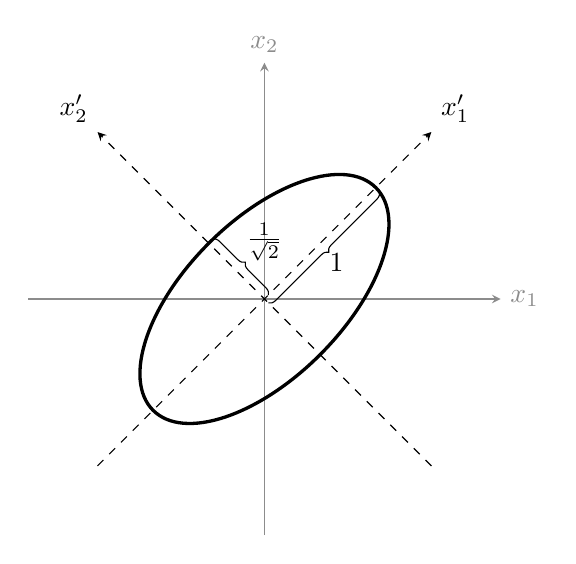
\begin{tikzpicture}[>=stealth]
        \draw[->, gray!90] (0, -3) -- (0, 3) node[above] {$x_2$};
        \draw[->, gray!90] (-3, 0) -- (3, 0) node[right] {$x_1$};

        \draw[very thick, rotate=-45] (0, 0) ellipse (1cm and 2cm);

        \draw[dashed, ->] (2.12, -2.12) -- (-2.12, 2.12) node[above left] {$x_2'$};
        \draw[decorate, decoration={brace, mirror, raise=2pt}] (0, 0) -- node[above right] {$\frac{1}{\sqrt{2}}$} (-0.71, 0.71);
        \draw[dashed, ->] (-2.12, -2.12) -- (2.12, 2.12) node[above right] {$x_1'$};
        \draw[decorate, decoration={brace, mirror, raise=2pt}] (0, 0) -- node[below right] {$1$} (1.41, 1.41);
      \end{tikzpicture}
      \end{center}
    \end{case}
    \begin{case}{Hyperbola}
      If we take
      \[
        \alpha = -\frac{1}{2},\ \beta = \frac{3}{2} \implies \lambda_1 = 1, \lambda_2 = -2
      \]
      Therefore:
      \[
        \mathcal{F}(\vec{x}) = (x_1')^2 - 2(x_2')^2 = 1
      \]
      Setting $\mathcal{F}(\vec{x}) = 1$ defines a hyperbola with respect to the principal axes:
      \begin{center}
      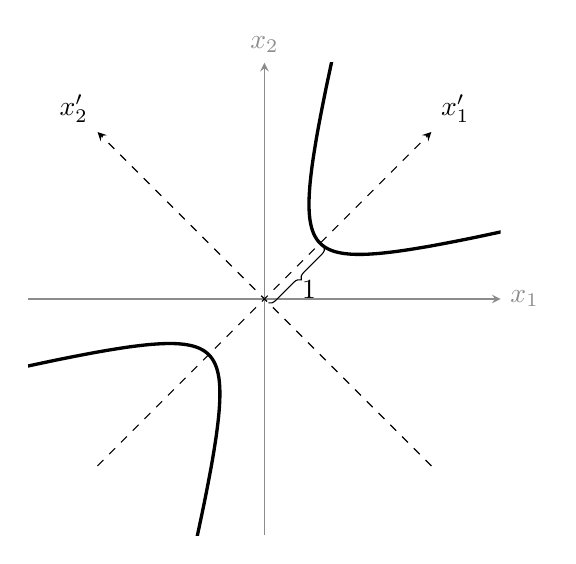
\begin{tikzpicture}[>=stealth]
        \draw[->, gray!90] (0, -3) -- (0, 3) node[above] {$x_2$};
        \draw[->, gray!90] (-3, 0) -- (3, 0) node[right] {$x_1$};

        \begin{scope}
          \clip (-3, -3) rectangle (3, 3);
          \draw[very thick, rotate=45, domain=-1.4:1.4, smooth, variable=\t] plot ({sec(\t r)},{0.6*tan(\t r)});
          \draw[very thick, rotate=-135, domain=-1.4:1.4, smooth, variable=\t] plot ({sec(\t r)},{0.6*tan(\t r)});
        \end{scope}

        \draw[dashed, ->] (2.12, -2.12) -- (-2.12, 2.12) node[above left] {$x_2'$};
        \draw[dashed, ->] (-2.12, -2.12) -- (2.12, 2.12) node[above right] {$x_1'$};
        \draw[decorate, decoration={brace, mirror, raise=2pt}] (0, 0) -- node[below right] {$1$} (0.71, 0.71);
      \end{tikzpicture}
      \end{center}
    \end{case}
  \end{proofcases}
\end{example}
\begin{example}[Quadratic Forms in 3D]
  If we diagonalise $\mathcal{F}$, we can write it using the coordinates with respect to the principal axes and the eigenvalues of $A$:
  \[
    \mathcal{F}(\vec{x}) = \vec{x}^{\trans} A \vec{x} = \lambda_1(x_1')^2 + \lambda_2 (x_2')^2 + \lambda_3 (x_3')^2
  \]
  \begin{proofcases}
    \begin{case}{$\lambda_1, \lambda_2, \lambda_3 > 0$}
      Setting $\mathcal{F(\vec{x})} = 1$ defines an ellipsoid aligned with the principal axes:
      \begin{center}
      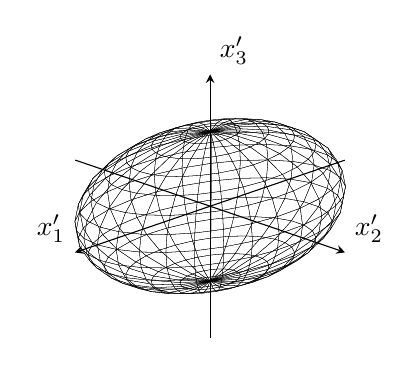
\begin{tikzpicture}
      \begin{axis}[
        view={135}{20},
        axis lines=center,axis on top,
        ticks=none,set layers=default,axis equal,
        xlabel={$x_1'$}, ylabel={$x_2'$}, zlabel={$x_3'$},
        xlabel style={anchor=south east},
        ylabel style={anchor=south west},
        zlabel style={anchor=south west},
        enlargelimits,
        tick align=inside,
        domain=0:2.00,
        samples=20,
        z buffer=sort,
      ]
        \def\a{3}
        \def\b{2}
        \def\c{1.5}

        \addplot3[
            mesh,
            samples=15,
            samples y=30,
            domain=-90:90,
            domain y=0:360,
            draw=black,
            line width=0.1pt,
        ]
        (
            { \a*cos(x)*cos(y) },
            { \b*cos(x)*sin(y) },
            { \c*sin(x) }
        );
      \end{axis}
      \end{tikzpicture}
      \end{center}
    \end{case}
    \begin{case}{$\lambda_1, \lambda_2, \lambda_3$ do not all have the same sign}
      For example, consider the matrix:
      \[
        A = \begin{pmatrix}
        0 & 1 & 1 \\
        1 & 0 & 1 \\
        1 & 1 & 0 \\
        \end{pmatrix}
        \implies \lambda_1 = \lambda_2 = - 1,\ \lambda_3 = 2
      \]
      We can then find the following orthonormal eigenvectors:
      \[
        \vec{u}_1 = \frac{1}{\sqrt{2}}\begin{pmatrix}
        1 \\
        -1 \\
        0 \\
        \end{pmatrix},\
        \vec{u}_2 = \frac{1}{\sqrt{6}}\begin{pmatrix}
        1 \\
        1 \\
        -2 \\
        \end{pmatrix},\
        \vec{u}_3 = \frac{1}{\sqrt{3}}\begin{pmatrix}
        1 \\
        1 \\
        1 \\
        \end{pmatrix}
      \]
      These are the principal axes of $\mathcal{F}$.

      We can then find $\mathcal{F}$ with respect to the standard axes and the principal axes:
      \begin{align*}
        \mathcal{F}(\vec{x}) &= 2x_1 x_2 + 2x_2x_3 + 2x_3 x_1 \\
                             &= -(x_1')^2 - (x_2')^2 + 2(x_3')^2
      \end{align*}
      Setting $\mathcal{F}(\vec{x}) = 1$ defines a hyperboloid with 2 sheets aligned with the principal axes:
      \begin{center}
      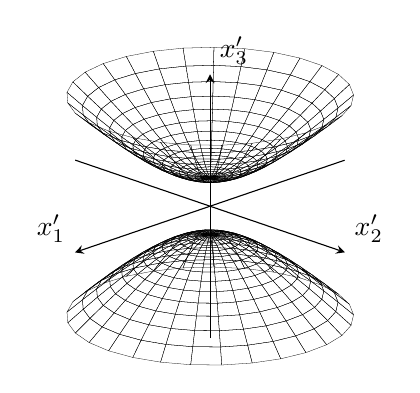
\begin{tikzpicture}
      \begin{axis}[
        view={135}{20},
        axis lines=center,axis on top,
        ticks=none,set layers=default,axis equal,
        xlabel={$x_1'$}, ylabel={$x_2'$}, zlabel={$x_3'$},
        xlabel style={anchor=south east},
        ylabel style={anchor=south west},
        zlabel style={anchor=south west},
        enlargelimits,
        tick align=inside,
        domain=0:2.00,
        samples=20,
        z buffer=sort,
      ]
        \def\a{0.5}
        \def\b{0.5}
        \def\c{0.5}
        \def\umax{1.4}

        \addplot3[
            mesh,
            samples=15,
            samples y=30,
            domain=0:\umax,
            domain y=0:360,
            draw=black,
            line width=0.1pt,
        ]
        (
            {\a*sinh(x)*cos(y)},
            {\b*sinh(x)*sin(y)},
            {\c*cosh(x) - 0.3}
        );

        \addplot3[
            mesh,
            samples=15,
            samples y=30,
            domain=0:\umax,
            domain y=0:360,
            draw=black,
            line width=0.1pt,
        ]
        (
            {\a*sinh(x)*cos(y)},
            {\b*sinh(x)*sin(y)},
            {-\c*cosh(x) + 0.3}
        );
      \end{axis}
      \end{tikzpicture}
      \end{center}
      Setting $\mathcal{F}(\vec{x}) = -1$ also defines a hyperboloid aligned with the principal axes but now with only one sheet:

      \begin{center}
      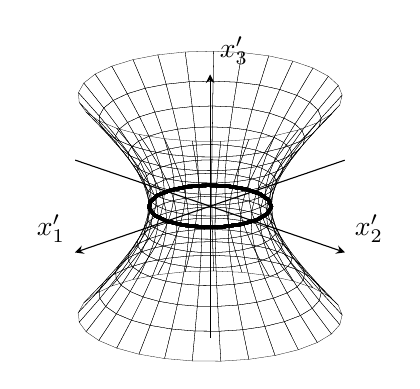
\begin{tikzpicture}
      \begin{axis}[
        view={135}{20},
        axis lines=center,axis on top,
        ticks=none,set layers=default,axis equal,
        xlabel={$x_1'$}, ylabel={$x_2'$}, zlabel={$x_3'$},
        xlabel style={anchor=south east},
        ylabel style={anchor=south west},
        zlabel style={anchor=south west},
        enlargelimits,
        tick align=inside,
        domain=0:2.00,
        samples=20,
        z buffer=sort,
      ]
        \def\a{0.5}
        \def\b{0.5}
        \def\c{0.5}
        \def\umax{1.4}

        \addplot3[
            mesh,
            samples=15,
            samples y=30,
            domain=-\umax:\umax,
            domain y=0:360,
            draw=black,
            line width=0.1pt,
        ]
        (
            {\a*cosh(x)*cos(y)},
            {\b*cosh(x)*sin(y)},
            {\c*sinh(x)}
        );
        \addplot3[
            mesh,
            domain=0:360,
            samples=20,
            very thick,
            black
        ]
        (
          { \a*cos(x) },
          { \b*sin(x) },
          { 0 }
        );
      \end{axis}
      \end{tikzpicture}
      \end{center}
      This cuts the plane $x_3' = 0$ in the circle $(x_1')^2 + (x_2')^2 = 1$.
    \end{case}
  \end{proofcases}
\end{example}
\begin{remark}
  Given a real square matrix $M$, we saw in \cref{matrixDecomp} that we can decompose $M$ into:
  \[
    M = S + A
  \]
  where $S$ is symmetric and $A$ is antisymmetric.

  Let $k = \vec{x}^{\trans}A\vec{x}$, then:
  \[
    k = \vec{x}^{\trans}A\vec{x} = (\vec{x}^{\trans}A^{\trans}\vec{x})^{\trans} = -(\vec{x}^{\trans}A\vec{x})^{\trans} = -k^{\trans} = -k \implies k=\vec{x}^{\trans}A\vec{x} = 0
  \]
  So for an antisymmetric matrix $A$, $\vec{x}^{\trans}A\vec{x} = 0$.
  Therefore:
  \[
    \vec{x}^{\trans} M \vec{x} = \vec{x}^{\trans}(S + A)\vec{x} = \vec{x}^{\trans}S\vec{x}
  \]
  This is why for quadratic forms we always use a symmetric matrix as if we used a general matrix, it could just be reduced to a quadratic form with a symmetric matrix.
\end{remark}
\section{Quadrics and Conics}
\subsection{Quadrics}
A \textit{quadric} in $\R^{n}$ is a hypersurface defined by:
\[
  Q(\vec{x}) = \vec{x}^{\trans}A\vec{x} + \vec{b}^{\trans}\vec{x} + c = 0
\]
for some real $n \times n$ real symmetric matrix $A$, $b \in \R^{n}$, and $c \in \R$.

We can also write $Q(\vec{x})$ in component form as:
\[
  Q(\vec{x}) = A_{i j}x_ix_j + b_i x_i + c = 0
\]

We now wish to classify solutions of this equation up to \textit{geometrical equivalence}, that is, we have no distinctions between solutions related by isometries in $\R^{n}$, i.e. we consider two solutions the same if they are related by:
\begin{itemize}
  \item Translations or changes in origin
  \item Orthogonal transformations about the origin
\end{itemize}
If $A$ is invertible, we can ``complete the square'' to simplify the equation.
Let $\vec{y} = \vec{x} + \frac{1}{2}A^{-1}\vec{b}$.
Noting that $A^{\trans} = A \implies A^{-1} A^{\trans} = I \implies (A^{-1})^{\trans} = A^{-1}$, we then have:
\[
  \vec{y}^{\trans} = \vec{x}^{\trans} + \frac{1}{2}\vec{b}^{\trans}A^{-1}
\]
We can then evaluate $\mathcal{F}(\vec{y})$ as:
\begin{align*}
  \mathcal{F}(\vec{y}) &= \vec{y}^{\trans}A\vec{y} \\
                       &= \vec{x}^{\trans}A\vec{x} + \vec{b}^{\trans} \vec{x} + \frac{1}{4}\vec{b}^{\trans}A^{-1}\vec{b} \\
                       &= \vec{x}^{\trans}A\vec{x} + \vec{b}^{\trans} \vec{x} + c +  \frac{1}{4}\vec{b}^{\trans}A^{-1}\vec{b} - c \\
                       &= Q(\vec{x}) + k
\end{align*}
where $k = \frac{1}{4}\vec{b}^{\trans} A^{-1} \vec{b} - c$.
Therefore:
\[
  \mathcal{F}(\vec{y}) = k \iff Q(\vec{x}) = 0
\]
Now, we diagonalise $\mathcal{F}$ as we did for the quadratic forms.
We know that the orthonormal eigenvectors give the principal axes, then the eigenvalues of $A$ along with the value of $k$ determine the geometrical nature of the quadric.
\subsubsection{Geometric Cases}
\begin{enumerate}
  \item Eigenvalues all positive and $k$ is positive $\to$ \textbf{Ellipsoid}
  \item Eigenvalues of mixed signs and $k \neq 0$ $\to$ \textbf{Hyperboloid}
  \item If $A$ has one or more zero eigenvalues, then $A$ is not invertible.
    We are unable to complete the square as we did above.
    It is simplest to continue analysis on a case by case basis using $Q(\vec{x})$ in its component form.
\end{enumerate}
\subsection{Conics}
Quadrics in $\R^2$ are curves called \textit{conics}.
\begin{proofcases}
  \begin{case}{$\det A \neq0$}
    Since $A$ is invertible, we can complete the square as above to obtain $\mathcal{F}(\vec{y}) = k$.
    After diagonalising, we obtain:
    \[
      \lambda_1 (y_1')^2 + \lambda_2 (y_2')^2 = k
    \]
    where $y_1'$ and $y_2'$ are coordinates with respect to the principal axes of $A$.
    Since $\vec{y}$ is $\vec{x}$ shifted by a constant vector, these axes will not necessarily be centred at the origin.
    \begin{proofcases}
      \begin{case}{$\lambda_1, \lambda_2 > 0$}
        \begin{itemize}
          \item For $k > 0$ $\to$ \textbf{Ellipse}
          \item For $k = 0$ $\to$ \textbf{Point}
          \item For $k < 0$ $\to$ \textbf{No solution}
        \end{itemize}
      \end{case}
      \begin{case}{$\lambda_1 > 0, \lambda_2 < 0$}
        \begin{itemize}
          \item For $k\neq0$ $\to$ \textbf{Hyperbola}
          \item For $k = 0$ $\to$ \textbf{Pair of lines}
        \end{itemize}
      \end{case}
    \end{proofcases}
  \end{case}
  \begin{case}{$\det A = 0$}
    As discussed, since $\det A = 0$ we cannot complete the square using $\vec{y}$ so instead we need to analyse $Q(\vec{x})$ directly.
    Since $\det A = 0$, we must have an eigenvalue of 0.

    Consider $\lambda_1 > 0$ and $\lambda_2 = 0$.
    After diagonalising $A$ in the original formula for $Q(\vec{x})$, we get:
    \begin{align*}
      \lambda_1(x_1')^2 + b_1'x_1' + b_2'x_2' + c &= 0 \\
      \lambda_1(x_1')^2 + b_1'x_1' + \frac{1}{4\lambda_1}(b_1')^2 - \frac{1}{4\lambda_1}(b_1')^2 + b_2'x_2' + c &= 0 \\
      \lambda_1\left(x_1' + \frac{1}{2\lambda_1}b_1'\right)^2 - \frac{1}{4\lambda_1}(b_1')^2 + b_2'x_2' + c &= 0 \\
      \lambda_1(x_1'')^2 + b_2'x_2' + c - \frac{1}{4 \lambda_{1}}(b_1')^2 &= 0 \\
      \lambda_1(x_1'')^2 + b_2'x_2' + c' &= 0
    \end{align*}
    where:
    \[
      x_1'' = x_1' + \frac{1}{2\lambda_1}b_1' \text{ and } c'=c-\frac{1}{4\lambda_1}(b_1')^2
    \]
    \begin{proofcases}
      \begin{case}{$b_2' = 0$}
        \begin{itemize}
          \item For $c' < 0$ $\to$ \textbf{Pair of parallel lines}
          \item For $c' = 0$ $\to$ \textbf{Single line}
          \item For $c' > 0$ $\to$ \textbf{No solution}
        \end{itemize}
      \end{case}
      \begin{case}{$b_2 \neq 0$}
        If we set:
        \[
          x_2'' = x_2' + \frac{1}{b_2' c'}
        \]
        then the equation becomes:
        \[
          \lambda_1(x_1'')^2 + b_2'x_2'' = 0
        \]
        which describes a parabola.
      \end{case}
    \end{proofcases}
  \end{case}
  Note that all changes of coordinates have been translations or orthogonal transformations about a given point.
  Therefore, all the transformations have preserved distances and angles so solutions are geometrically equivalent. 
\end{proofcases}
\subsubsection{Standard Forms for Conics in Cartesian Coordinates}
\begin{proofcases}
  \begin{case}{Ellipse}
    Consider the equation:
    \[
      \frac{x^2}{a^2} + \frac{y^2}{b^2} = 1
    \]
    This matches with the case above where both eigenvalues are positive and $k > 0$ so we get an ellipse.
    \begin{center}
    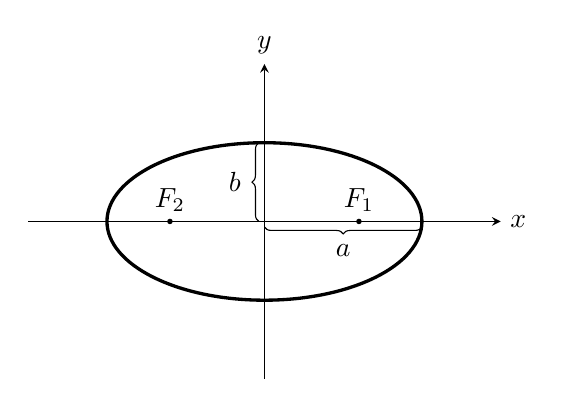
\begin{tikzpicture}[>=stealth]
      \draw[->] (0, -2) -- (0, 2) node[above] {$y$};
      \draw[->] (-3, 0) -- (3, 0) node[right] {$x$};

      \draw[very thick] (0, 0) ellipse (2cm and 1cm);

      \draw[decorate, decoration={brace, mirror, raise=2pt}] (0, 0) -- node[below=5pt] {$a$} (2, 0);
      \draw[decorate, decoration={brace, raise=2pt}] (0, 0) -- node[left=5pt] {$b$} (0, 1);

      \fill (1.2, 0) circle (1pt) node[above] {$F_1$};
      \fill (-1.2, 0) circle (1pt) node[above] {$F_2$};
    \end{tikzpicture}
    \end{center}
    Where $a$ is the \textit{semi-major axis} and $b$ is the \textit{semi-minor axis}.

    Ellipses have \textit{eccentricity}, $e < 1$.
    For $a > b$, $b^2 = a^2(1 - e^2)$ and they have foci at $(\pm ae, 0)$
  \end{case}
  \begin{case}{Parabola}
    Parabola have general equation:
    \[
      y^2 = 4ax
    \]
    where $a > 0$.

    They have eccentricity $e = 1$ and have a single focus at $x = a$.

    \begin{center}
    \begin{tikzpicture}[>=stealth]
      \draw[->] (0, -2) -- (0, 2) node[above] {$y$};
      \draw[->] (-3, 0) -- (3, 0) node[right] {$x$};

      \clip (-3, -3) rectangle (3, 3);
      \draw[very thick, rotate=-90,domain=-2:2, samples=50] plot ({\x}, {(\x)^2});

      \fill (1.2, 0) circle (1pt) node[above] {$F$} node[below] {\small$(a, 0)$};
    \end{tikzpicture}
    \end{center}
  \end{case}
  \begin{case}{Hyperbola}
    Hyperbola have general equation:
    \[
      \frac{x^2}{a^2} - \frac{y^2}{b^2} = 1
    \]
    They have eccentricity $e > 1$, where:
    \[
      b^2 = a^2(e^2 - 1)
    \]
    They have foci at $x = \pm ae$ and asymptotes $y = \pm \frac{b}{a}x$.

    \begin{center}
    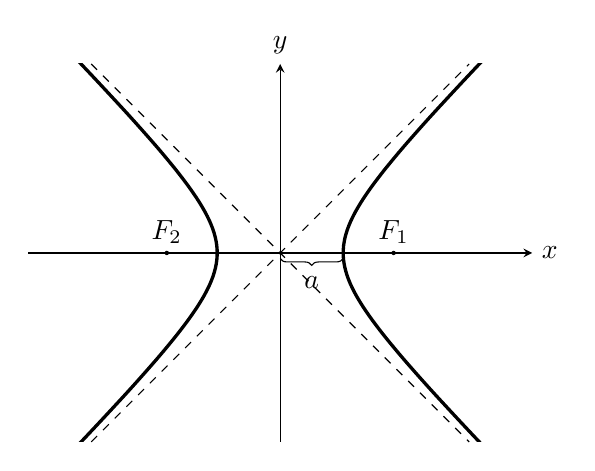
\begin{tikzpicture}[>=stealth, scale=0.8]
      \draw[->] (0, -3) -- (0, 3) node[above] {$y$};
      \draw[->] (-4, 0) -- (4, 0) node[right] {$x$};

      \begin{scope}
        \clip (-4, -3) rectangle (4, 3);
        \draw[very thick, domain=-1.4:1.4, smooth, variable=\t] plot ({sec(\t r)},{tan(\t r)});
        \draw[very thick, rotate=180, domain=-1.4:1.4, smooth, variable=\t] plot ({sec(\t r)},{tan(\t r)});
      \end{scope}

      \draw[decorate, decoration={brace, mirror, raise=2pt}] (0, 0) -- node[below=5pt] {$a$} (1, 0);

      \draw[dashed] (-3, -3) -- (3, 3);
      \draw[dashed] (-3, 3) -- (3, -3);

      \fill (1.8, 0) circle (1pt) node[above] {$F_1$};
      \fill (-1.8, 0) circle (1pt) node[above] {$F_2$};
    \end{tikzpicture}
    \end{center}
  \end{case}
\end{proofcases}
\subsubsection{Focus Directrix Property}
The 4 conic sections (circle, parabola, hyperbola, and ellipse) can be obtained by intersecting a plane at varying angles with a double cone:
\begin{itemize}
  \item Plane \textbf{horizontal} $\to$ \textbf{Circle}
  \item Plane \textbf{parallel to the slant} of the cone $\to$ \textbf{Parabola}
  \item Plane \textbf{vertical} $\to$ \textbf{Hyperbola} (only one which intersects both cones simultaneously)
  \item Otherwise $\to$ \textbf{Ellipse}
\end{itemize}
\begin{definition}[Conic Sections]
  For all \textit{conic sections} or \textit{conics}, we define the following for a positive real scale parameter $a$:
  \begin{itemize}
    \item The \textit{eccentricity} of a conic is a non-negative parameter $e$.
    \item The \textit{foci} of a conic are at $(\pm ae, 0)$.
    \item The \textit{directrices} of a conic are the lines $x = \pm \frac{a}{e}$
  \end{itemize}
  A conic is then the set of points whose distance from the focus is $e$ times the distance from the directrix which is closest to that focus (With the exception of $e = 1$, in which case, we take the distance to the other further directrix).

  This is known as the \textit{focus-directrix property}.
\end{definition}
\begin{proofcases}
  \begin{case}{$e < 1$ -- Ellipse or Circle}
    When $e < 1$ we obtain an ellipse:

    \begin{center}
    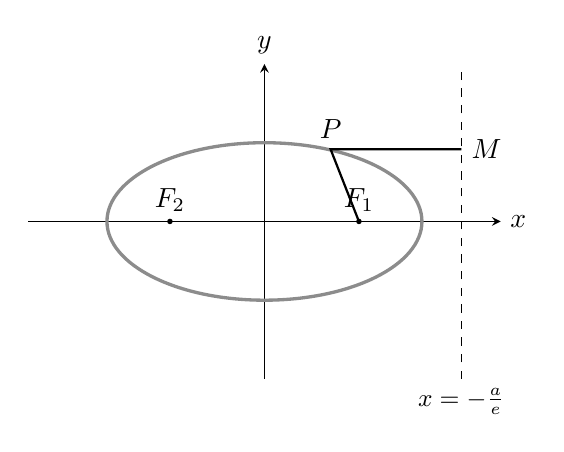
\begin{tikzpicture}[>=stealth]
      \draw[->] (0, -2) -- (0, 2) node[above] {$y$};
      \draw[->] (-3, 0) -- (3, 0) node[right] {$x$};

      \draw[very thick, gray!90] (0, 0) ellipse (2cm and 1cm);


      \fill (1.2, 0) circle (1pt) node[above] {$F_1$};
      \fill (-1.2, 0) circle (1pt) node[above] {$F_2$};

      \draw[dashed] (2.5, -2) node[below] {\small$x = -\frac{a}{e}$} -- (2.5, 2);
      \draw[thick] (1.2, 0) -- (0.84, 0.917) node[above] {$P$} -- (2.5, 0.917) node[right] {$M$};
    \end{tikzpicture}
    \end{center}
    We must have $|PF| = e|PM|$ and so we obtain:
    \[
      \sqrt{(x - ae)^2 + y^2} = e\left(\frac{a}{e} - x\right) \implies
      \frac{x^2}{a^2} + \frac{y^2}{a^2(1 - e^2)} = 1
    \]
    with $b = a\sqrt{1 - e^2}$.
    In the limiting case as $e \to 0$, we have a circle.
  \end{case}
  \begin{case}{$e > 1$}
    When $e > 1$ we obtain a hyperbola:
    \begin{center}
    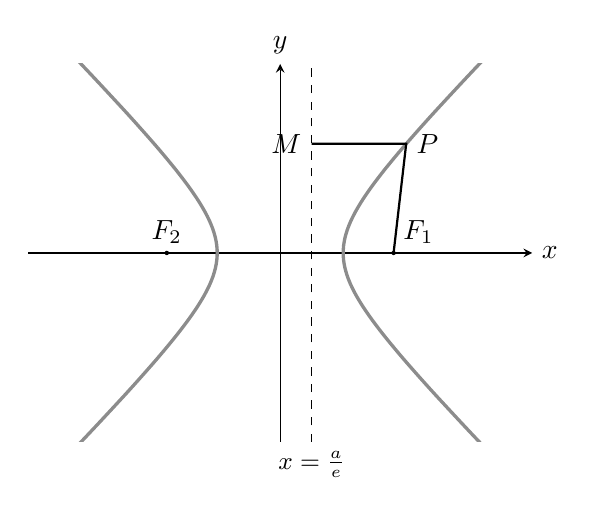
\begin{tikzpicture}[>=stealth, scale=0.8]
      \draw[->] (0, -3) -- (0, 3) node[above] {$y$};
      \draw[->] (-4, 0) -- (4, 0) node[right] {$x$};

      \begin{scope}
        \clip (-4, -3) rectangle (4, 3);
        \draw[very thick, domain=-1.4:1.4, smooth, variable=\t, gray!90] plot ({sec(\t r)},{tan(\t r)});
        \draw[very thick, rotate=180, domain=-1.4:1.4, smooth, variable=\t, gray!90] plot ({sec(\t r)},{tan(\t r)});
      \end{scope}

      \draw[dashed] (0.5, -3) node[below] {\small$x = \frac{a}{e}$} -- (0.5, 3);
      \fill (1.8, 0) circle (1pt) node[above right] {$F_1$};
      \fill (-1.8, 0) circle (1pt) node[above] {$F_2$};

      \draw[thick] (1.8, 0) -- (2, 1.732) node[right] {$P$} -- (0.5, 1.732) node[left] {$M$};
    \end{tikzpicture}
    \end{center}
    We must have $|PF| = e|PM|$ and so we obtain:
    \[
      \sqrt{(x - ae)^2 + y^2} = e\left(x - \frac{a}{e}\right) \implies
      \frac{x^2}{a^2} - \frac{y^2}{a^2(e^2 - 1)} = 1
    \]
    with $b = a\sqrt{e^2 - 1}$.
  \end{case}
  \begin{case}{$e = 1$}
    \begin{center}
    \begin{tikzpicture}[>=stealth]
      \draw[->] (0, -2) -- (0, 2) node[above] {$y$};
      \draw[->] (-3, 0) -- (3, 0) node[right] {$x$};

      \clip (-3, -3) rectangle (3, 3);
      \draw[very thick, rotate=-90,domain=-2:2, samples=50, gray!90] plot ({\x}, {(\x)^2});

      \fill (1, 0) circle (1pt) node[above] {$F$} node[below] {\small$(a, 0)$};

      \draw[dashed] (-0.25, -2) node[below] {\small$x = -\frac{a}{e}$} -- (-0.25, 2);
      \draw[thick] (1, 0) -- (1.2, 1.095) node[above] {$P$} -- (-0.25, 1.095) node[left] {$M$};
    \end{tikzpicture}
    \end{center}
    We must have $|PF| = |PM|$ and so we obtain
    \[
      \sqrt{(x - a)^2 + y^2} = (x + a) \implies y^2 = 4ax
    \]
  \end{case}
\end{proofcases}
\subsubsection{Conics in Polar Coordinates}
We introduce a new parameter the \textit{semi-latus rectum}, $\ell$, such that $\frac{\ell}{e}$ is the distance from the focus to the appropriate directrix.

In the case of $e \neq 1$, we use the closet directrix so have:
\[
  \frac{\ell}{e} = \abs{\frac{a}{e} - ae} \implies \ell = a|1 - e^2|
\]
In the case $e = 1$ (parabola), we use the other directrix so $\ell = 2a$.

We use polar coordinates $(r, \theta)$ that are centered on a focus:
\begin{center}
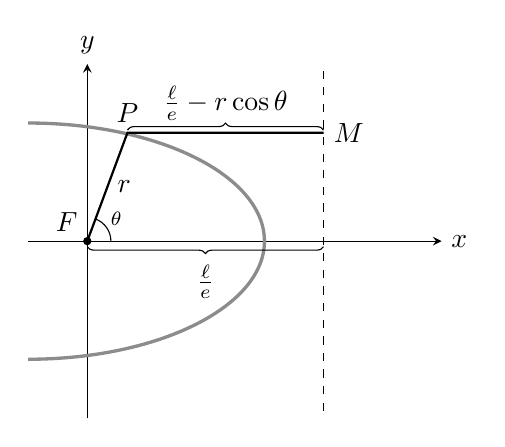
\begin{tikzpicture}[>=stealth, scale=1.5]
  \draw[->] (0, -1.5) -- (0, 1.5) node[above] {$y$};
  \draw[->] (-0.5, 0) -- (3, 0) node[right] {$x$};

  \begin{scope}[xshift=-0.5cm]
    \clip (0, -1.5) rectangle (3, 1.5);
    \draw[very thick, gray!90] (0, 0) ellipse (2cm and 1cm);
    \fill (0.5, 0) circle (1pt) node[above left] {$F$};

    \draw[decorate, decoration={brace, mirror,raise=2pt}] (0.5, 0) -- node[below=5pt] {$\frac{\ell}{e}$} (2.5, 0);

    \draw (0.7,0) arc[start angle=0, end angle=70, radius=0.2] node[right, xshift=2] {$\scriptstyle\theta$};

    \draw[dashed] (2.5, -2) -- (2.5, 2);
    \draw[thick] (0.5, 0) -- (0.84, 0.917) node[midway, right] {$r$} node[above] {$P$} -- (2.5, 0.917) node[right] {$M$};
    \draw[decorate, decoration={brace, raise=1pt}] (0.84, 0.917) -- node[above=1pt] {$\frac{\ell}{e} - r\cos\theta$} (2.5, 0.917);
  \end{scope}
\end{tikzpicture}
\end{center}
Hence, the focus-directrix property is given by:
\[
  r = e\left(\frac{\ell}{e} - r\cos \theta\right) \implies r= \frac{\ell}{1 + e\cos \theta}
\]
\begin{proofcases}
  \begin{case}{$e < 1$ -- Ellipse}
    In this case we have $\ell = a(1 - e^2)$ so $r = \frac{a(1 - e^2)}{1 + e\cos \theta}$.

    \begin{center}
    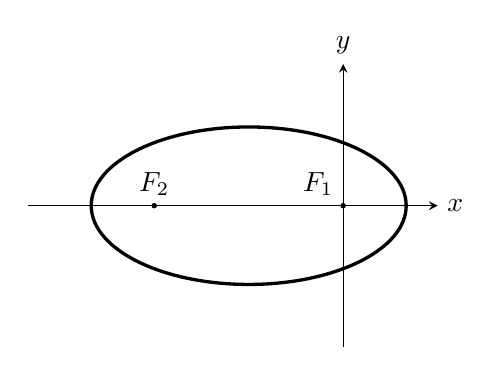
\begin{tikzpicture}[>=stealth]
      \draw[->] (0, -1.8) -- (0, 1.8) node[above] {$y$};
      \draw[->] (-4, 0) -- (1.2, 0) node[right] {$x$};

      \begin{scope}[xshift=-1.2cm]
        \draw[very thick] (0, 0) ellipse (2cm and 1cm);
        \fill (1.2, 0) circle (1pt) node[above left] {$F_1$};
        \fill (-1.2, 0) circle (1pt) node[above] {$F_2$};
      \end{scope}
    \end{tikzpicture}
    \end{center}
  \end{case}
  \begin{case}{$e = 1$ -- Parabola}
    Since $e = 1$, we have $\ell = 2a$ so $r = \frac{2a}{1 + e\cos \theta}$.
    \begin{center}
    \begin{tikzpicture}[>=stealth]
      \draw[->] (0, -2) -- (0, 2) node[above] {$y$};
      \draw[->] (-3, 0) -- (1.8, 0) node[right] {$x$};

      \clip (-3, -3) rectangle (3, 3);
      \begin{scope}[xshift=1.2cm]
        \draw[very thick, rotate=90,domain=-2:2, samples=50] plot ({\x}, {(\x)^2});

        \fill (-1.2, 0) circle (1pt) node[above left] {$F$};
      \end{scope}
    \end{tikzpicture}
    \end{center}
  \end{case}
  \begin{case}{$e > 1$ -- Hyperbola}
    In this case we have $\ell = a(e^2 - 1)$ so $r = \frac{a(e^2 - 1)}{1 + e\cos \theta}$.
    \begin{center}
    \begin{tikzpicture}[>=stealth, scale=0.8]
      \draw[->] (0, -3) -- (0, 3) node[above] {$y$};
      \draw[->] (-3, 0) -- (3, 0) node[right] {$x$};

      \clip (-4, -3) rectangle (4, 3);
      \begin{scope}[xshift=1.8cm]
        \draw[very thick, rotate=180, domain=-1.4:1.4, smooth, variable=\t] plot ({sec(\t r)},{tan(\t r)});
        \draw[dashed] (-3, 3) -- (0, 0) -- (-3, -3);
        \fill (-1.8, 0) circle (1pt) node[above left] {$F$};
      \end{scope}
    \end{tikzpicture}
    \end{center}
  \end{case}
\end{proofcases}
\section{Jordan Canonical/Normal Forms}
This gives us a classification for $n \times n$ complex matrices up to similarity.

Consider an $n \times n$ matrix $A$ corresponding to a linear map $T: \C^{n} \to \C^{n}$ which is similar to the matrix $B$ after a change of basis.
\begin{proposition}[Jordan normal forms in $\C^2$]
  \label{2x2Similar}
  Let $A$ be a $2 \times 2$ complex matrix $A$ with eigenvalues $\lambda_1$ and $\lambda_2$:
  \begin{enumerate}
    \item If $\lambda_1 \neq \lambda_2$, then $A$ is similar to:
      \[
        B = \begin{pmatrix}
        \lambda_1 & 0 \\
        0 & \lambda_2 \\
        \end{pmatrix}
      \]
    \item If $\lambda_1 = \lambda_2 = \lambda$ and $m_\lambda = 2$, then $A$ is similar to:
      \[
        B = \begin{pmatrix}
        \lambda & 0 \\
        0 & \lambda \\
        \end{pmatrix}
      \]
    \item If $\lambda_1 = \lambda_2 = \lambda$ and $m_\lambda = 1$, then $A$ is similar to:
      \[
        B = \begin{pmatrix}
        \lambda & 1 \\
        0 & \lambda \\
        \end{pmatrix}
      \]
  \end{enumerate}
\end{proposition}
\begin{proof}
  We know that $\chi_A(t)$ has 2 roots, counting multiplicity over $\C$.
  \begin{enumerate}
    \item For distinct roots/eigenvalues $\lambda_1, \lambda_2$, we have:
      \[
        M_{\lambda_1} = m_{\lambda_1} = 1 \text{ and } M_{\lambda_2} = m_{\lambda_2} = 1
      \]
      Since the algebraic and geometric multiplicities coincide for all eigenvalues, by \cref{diagonalisationIFF}, $A$ can be diagonalised by the matrix $P$ that has its eigenvectors as its columns.

      Therefore, we have $P^{-1}AP = B$ for a diagonal matrix $B$.
      So $A$ is similar to
      \[
        B = \begin{pmatrix}
        \lambda_1 & 0 \\
        0 & \lambda_2 \\
        \end{pmatrix}
      \]
    \item For $\lambda_1 = \lambda_2 = \lambda$ and $M_\lambda = m_{\lambda} = 2$ we can diagonalise so the same argument applies.
    \item For $\lambda_1 = \lambda_2 = \lambda$ and $M_\lambda = 2 \neq m_{\lambda} = 1$, let $\vec{v}$ be an eigenvector for $\lambda$ and extend this to a basis for $\C^{2}$ by adjoining a vector $\vec{w}$ that is linearly independent to $\vec{v}$.

      Since $\vec{v}$ is an eigenvector, $A \vec{v} = \lambda \vec{v}$.
      We can also write:
      \[
        A\vec{w} = \alpha \vec{v} + \beta \vec{w}
      \]
      to represent $A\vec{w}$ in the basis $\{\vec{v}, \vec{w}\}$.
      Note that $\alpha \neq 0$ as we cannot have a second linearly independent eigenvector.

      Then, the matrix representing the linear map $T$ with respect to the basis $\{\vec{v}, \vec{w}\}$ is:
      \[
        \begin{pmatrix}
        \lambda & \alpha \\
        0 & \beta \\
        \end{pmatrix}
      \]
      This matrix must be similar to $A$ as it represents the same transform in a different basis.
      It therefore needs to have the same repeated eigenvalue $\lambda$ so we require that $\beta = \lambda$.

      Now defining $\vec{u} = \alpha \vec{v}$, we have that:
      \[
        B = \begin{pmatrix}
        \lambda & 1 \\
        0 & \lambda \\
        \end{pmatrix}
      \]
      represents $T$ with respect to the basis $\{\vec{u}, \vec{w}\}$ as $A\vec{u} = \lambda \vec{u}$ and $A\vec{w} = \vec{u} + \lambda \vec{w}$.
      Therefore, $B = P^{-1} A P$ where $\vec{u}, \vec{w}$ are the columns of $P$.
      So $A$ is similar to $B$.
  \end{enumerate}
\end{proof}
\begin{theorem}[Jordan normal forms in $\C^n$]
  Any $n \times n$ complex matrix $A$ is similar to a matrix $B$ with block form given by:
  \[
    B = \begin{pmatrix}
    \multicolumn{1}{c|}{J_{n_1}(\lambda_1)} &  &  &  \\ \cline{1-2}
     & \multicolumn{1}{|c|}{J_{n_2}(\lambda_2)} &  &  \\ \cline{2-2}
     &  & \ddots &  \\ \cline{4-4}
     &  &  & \multicolumn{1}{|c}{J_{n_r}(\lambda_r)} \\
    \end{pmatrix}
  \]
  where all other entries are 0, $n_1 + \cdots n_r = n$, and $\lambda_1, \ldots, \lambda_r$ are eigenvalues of $A$ and $B$.

  Each \textit{Jordan block} $J_p(\lambda)$ is a $p \times p$ matrix of the form:
  \[
    J_p(\lambda) = \begin{pmatrix}
    \lambda & 1 &  &  &  \\
     & \lambda & 1 &  &  \\
     &  & \lambda & 1 &  \\
     &  &  & \ddots &  1\\
     &  &  &  & \lambda \\
    \end{pmatrix}
  \]
  where the main diagonal has only $\lambda$, the diagonal above has only $1$, and everything else is 0.
\end{theorem}
\begin{remark}[Note]
  The same eigenvalue may appear in more than one block.

  For example, considering the matrices in \cref{2x2Similar}:
  \begin{enumerate}
    \item We have 2 Jordan blocks with different eigenvalues.
    \item We have 2 Jordan Blocks with the same eigenvalue.
    \item The entire matrix is a single Jordan block.
  \end{enumerate}
\end{remark}
\begin{remark}
  $A$ is diagonalisable if and only if $B$ consists of only $1 \times 1$ Jordan blocks.
\end{remark}
\section{Symmetries and Transformation Groups}
\subsection{Orthogonal Transformations and Rotations}
Since we are talking about orthogonal matrices instead of unitary matrices, we will work in $\R^{n}$.
\begin{remark}[Recap] (See \cref{orthogonalMatrices} for full details)

  The following statements are equivalent:
  \begin{itemize}
    \item A square matrix $R$ is orthogonal.
    \item $R^{\trans} R = R R^{\trans} = I$.
    \item $(R \vec{x})\cdot(R \vec{y}) = \vec{x} \cdot \vec{y}\ \forall \vec{x}, \vec{y} \in \R^{n}$, that is, $R$ preserves lengths and angles.
    \item The columns of $R$ form an orthonormal basis.
  \end{itemize}
\end{remark}
\begin{definition}[Orthogonal Group]
  The set of orthogonal matrices $R$ of size $n \times n$, denoted by $O(n)$ is called the \textit{orthogonal group}.
\end{definition}
Recall from \cref{orthoDeterminant} that $R \in O(n) \implies \det R = \pm 1$.
\begin{definition}[Special Orthogonal Group]
  The subgroup of $O(n)$ formed by orthogonal matrices with $\det R = 1$ is called the \textit{special orthogonal group} and is denoted $\SO(n)$
\end{definition}
We already saw that $R \in O(n)$ preserve length, angles and the unsigned value of $n$-dimensional volumes.
However, matrices $R \in \SO(n)$ also preserve \textit{orientation}.
This means they preserve the signs of $n$-dimensional volumes.

The group $\SO(n)$ consists of all rotation in $\R^{n}$.
Reflections belong to $O(n)$ but not $\SO(n)$, so for any rotation $H$, $H \in O(n) \setminus \SO(n)$.

We can write any element of $O(n)$ in the form:
\begin{align*}
  &R \text{ where }R \in \SO(n) \\
  \text{ or }&RH \text{ where } R \in \SO(n),\ H \in O(n) \setminus \SO(n)
\end{align*}
For a rotation matrix $R$, we can find the components of the image of $\vec{x}$ using:
\[
  x_i' = R_{i j}x_j
\]
So far, we have been thinking of this a transformation of vectors.
This is called the \textit{active} point of view.
We typically take the standard basis $\{\vec{e}_1, \vec{e}_2\}$, and by means of the above transformation, we transform it to some $\vec{x}'$.
Since this is an orthogonal transformation, $|\vec{x}| = |\vec{x}'|$.
In this perspective, the components of both $\vec{x}$ and $\vec{x}'$ are both with respect to the standard basis.
\begin{center}
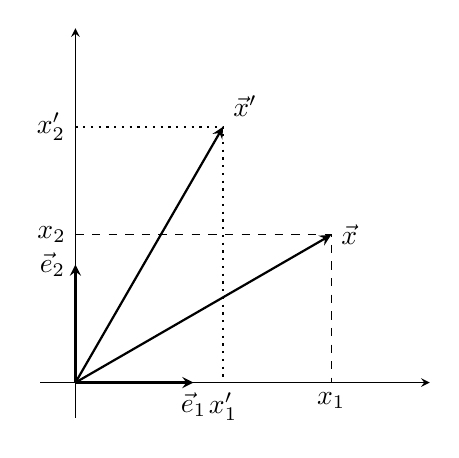
\begin{tikzpicture}[>=stealth, scale=1.5]
  \draw[->] (0, -0.3) -- (0, 3);
  \draw[->] (-0.3, 0) -- (3, 0);

  \draw[rotate=30, ->, thick] (0, 0) -- (2.5, 0) node[right] {$\vec{x}$};
  \draw[dashed] (0, 1.25) node[left] {$x_2$} -- (2.165, 1.25) -- (2.165, 0) node[below] {$x_1$};
  \draw[rotate=60, ->, thick] (0, 0) -- (2.5, 0) node[above right] {$\vec{x}'$};
  \draw[thick, dotted] (0, 2.165) node[left] {$x_2'$} -- (1.25, 2.165) -- (1.25, 0) node[below] {$x_1'$};

  \draw[->, thick] (0, 0) -- (1, 0) node[below] {$\vec{e}_1$};
  \draw[->, thick] (0, 0) -- (0, 1) node[left] {$\vec{e}_2$};
\end{tikzpicture}
\end{center}

However, we could also think of this orthogonal transformation as a change of basis, this is the \textit{passive} point of view.
If we keep the vector $\vec{x}$ fixed and instead change the basis, the components of $\vec{x}$ become $x_i'$ with respect to a different orthonormal basis $\{\vec{u}_1, \vec{u}_2\}$.
\begin{center}
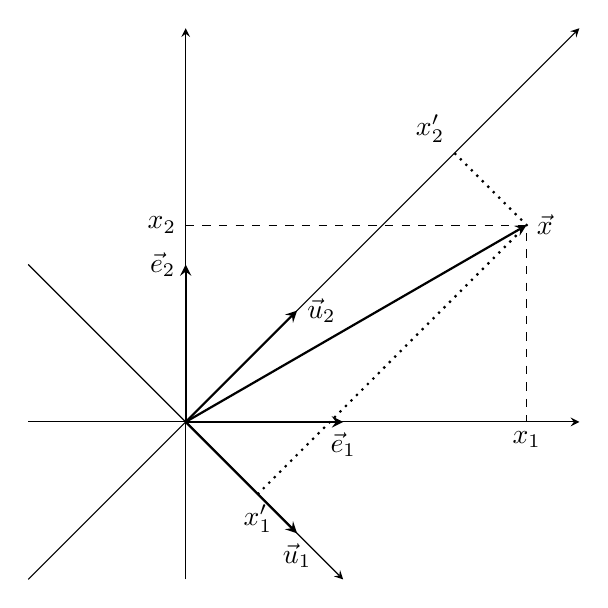
\begin{tikzpicture}[>=stealth, scale=2]
  \draw[->] (0, -1) -- (0, 2.5);
  \draw[->] (-1, 0) -- (2.5, 0);

  \draw[rotate=30, ->, thick] (0, 0) -- (2.5, 0) node[right] {$\vec{x}$};
  \draw[dashed] (0, 1.25) node[left] {$x_2$} -- (2.165, 1.25) -- (2.165, 0) node[below] {$x_1$};

  \draw[thick, dotted] (1.707, 1.707) node[above left] {$x_2'$} -- (2.165, 1.25) -- (0.458, -0.458) node[below] {$x_1'$};

  \draw[->, thick] (0, 0) -- (1, 0) node[below] {$\vec{e}_1$};
  \draw[->, thick] (0, 0) -- (0, 1) node[left] {$\vec{e}_2$};


  \draw[->, thick, rotate=-45] (0, 0) -- (1, 0) node[below] {$\vec{u}_1$};
  \draw[->, thick, rotate=-45] (0, 0) -- (0, 1) node[right] {$\vec{u}_2$};

  \draw[->] (-1, -1) -- (2.5, 2.5);
  \draw[->] (-1, 1) -- (1, -1);
\end{tikzpicture}
\end{center}
To get the transformed $\vec{x}$ in the original basis, we first determine the new basis $\{\vec{u}_1, \vec{u}_2\}$ with respect to the original basis as we did in \cref{changeOfBasis} and then use this to find the image:
\[
  \vec{u}_i = \sum_{j} R_{i j}\vec{e}_j = \sum_{j} \vec{e}_j (R^{-1})_{j i}
\]
where $R_{i j} = (R^{\trans})_{j i} = (R^{-1})_{j i}$ as $R$ is orthogonal.
\begin{remark}
  If we compare this to the standard rotation for the matrix of change of basis, we see that the change of basis matrix is $P = R^{-1}$.
  That is, we can either carry out the rotation directly in the active point of view, or transform the axes by the inverse rotation ($\vec{u}_i = P^{-1}\vec{e}_i$) and find the coordinates of $\vec{x}$ with respect to this new basis in the passive point of view.
\end{remark}
\subsection{2D Minkowski Space and Lorentz Transformations}
Consider a new ``inner product'' on $\R^2$ given by:
\[
  (\vec{x}, \vec{y}) = \vec{x}^{\trans} J \vec{y},\ J = \begin{pmatrix}
  1 & 0 \\
  0 & -1 \\
  \end{pmatrix}
\]
We can write this in terms of the components of $\vec{x}$ and $\vec{y}$:
\[
  \vec{x} = \begin{pmatrix}
  x_0 \\
  x_1 \\
  \end{pmatrix},\
  \vec{y} = \begin{pmatrix}
  y_0 \\
  y_1 \\
  \end{pmatrix} \implies (\vec{x}, \vec{y}) = x_0 y_0 - x_1 y_1
\]
We saw this originally in \cref{scalarCrossProduct}.

Note that this ``inner product'' is \textbf{not} positive definite as $(\vec{x}, \vec{x})$ is not necessarily positive.
However, it is still bilinear and symmetric (See \cref{innerProd} for details of the normal inner product on $\R^{2}$).

Consider the vectors $\vec{e}_0 = \begin{pmatrix}
1 \\
0 \\
\end{pmatrix}$ and $\vec{e}_1 = \begin{pmatrix}
0 \\
1 \\
\end{pmatrix}$.
Notice that:
\begin{align*}
  (\vec{e}_0, \vec{e}_0) &= 1 \\
  (\vec{e}_1, \vec{e}_1) &= -1 \\
  (\vec{e}_0, \vec{e}_1) & = 0
\end{align*}
This is similar to how basis vectors are orthonormal when using the standard inner product.
We generalise the notion of orthonormality to this new ``inner product'' as above so that the standard basis vectors are orthonormal in this metric.
\begin{definition}[Minkowski Space]
  The inner product defined for all $\vec{x}, \vec{y} \in \R^2$ by $\vec{x}^{\trans}J\vec{y}$ is called the \textit{Minkowski metric}.

  Futhermore, $\R^2$ equipped with the Minkowski metric is called the \textit{Minkowski space}.
\end{definition}
Consider a matrix associated with a linear map $T: \R^2 \to R^2$ of the form:
\[
  M = \begin{pmatrix}
  M_{0 0} & M_{0 1} \\
  M_{1 0} & M_{1 1} \\
  \end{pmatrix}
\]
We say that this matrix preserves the Minkowski metric if and only if:
\begin{align*}
  &(M\vec{x}, M\vec{y}) = (\vec{x}, \vec{y})\ \forall \vec{x}, \vec{y} \in \R^2 \\
  \iff& (M\vec{x})^{\trans}J(M\vec{y}) = \vec{x}^{\trans}J\vec{y} \ \forall \vec{x}, \vec{y} \in \R^2 \\
  \iff& \vec{x}^{\trans}(M^{\trans}JM)\vec{y} = \vec{x}^{\trans}J\vec{y} \ \forall \vec{x}, \vec{y} \in \R^2 \\
  \iff& M^{\trans}JM = J
\end{align*}
The matrices $M$ for which this holds form a group.
If we take determinants of each side, we see that matrices in this group must necessarily have $\det M = \pm 1$:
\[
  \det (M^{\trans})\det(J)\det(M) = \det(J) \implies (\det M)^2 = 1 \implies \det M = \pm 1
\]
\begin{definition}[Lorentz Group]
  The \textit{Lorentz group} is the subgroup of the group above for which $\det M = 1$ and $M_{0 0} > 0$.
\end{definition}

\textbf{General form of M}\par
To find the general form of a matrix $M$ in the Lorentz group, we will use a method similar to when we determined the general form of orthogonal matrices in $\R^2$ in \cref{orthoExampleR2}.

First, we use the fact that $(\vec{e}_0, \vec{e}_0) = 1$, so if $M$ is to preserve the Minkowski metric, we must have $(M\vec{e}_0, M\vec{e}_0) = 1$.
Thus:
\[
  \vec{e}^{\trans}_0 M^{\trans} J M \vec{e}_0 =
  (1, 0)\begin{pmatrix}
  M_{0 0} & M_{1 0} \\
  M_{0 1} & M_{1 1} \\
  \end{pmatrix}
  \begin{pmatrix}
  1 & 0 \\
  0 & -1 \\
  \end{pmatrix}
  \begin{pmatrix}
  M_{0 0} & M_{0 1} \\
  M_{1 0} & M_{1 1} \\
  \end{pmatrix}
  \begin{pmatrix}
  1 \\
  0 \\
  \end{pmatrix} = M_{0 0}^2 - M_{1 0}^2 = 1
\]
Similarly, since $(\vec{e}_1, \vec{e}_1) = -1$, we must have $(M\vec{e}_1, M\vec{e}_1) = -1$:
\[
  \vec{e}^{\trans}_1 M^{\trans} J M \vec{e}_1 =
  (0, 1)\begin{pmatrix}
  M_{0 0} & M_{1 0} \\
  M_{0 1} & M_{1 1} \\
  \end{pmatrix}
  \begin{pmatrix}
  1 & 0 \\
  0 & -1 \\
  \end{pmatrix}
  \begin{pmatrix}
  M_{0 0} & M_{0 1} \\
  M_{1 0} & M_{1 1} \\
  \end{pmatrix}
  \begin{pmatrix}
  0 \\
  1 \\
  \end{pmatrix} = M_{0 1}^2 - M_{1 1}^2 = -1
\]
Now using $(\vec{e}_0, \vec{e}_1) = 0$, so $(M\vec{e}_0, M\vec{e}_1) = 0$:
\[
  \vec{e}^{\trans}_0 M^{\trans} J M \vec{e}_1 =
  (1, 0)\begin{pmatrix}
  M_{0 0} & M_{1 0} \\
  M_{0 1} & M_{1 1} \\
  \end{pmatrix}
  \begin{pmatrix}
  1 & 0 \\
  0 & -1 \\
  \end{pmatrix}
  \begin{pmatrix}
  M_{0 0} & M_{0 1} \\
  M_{1 0} & M_{1 1} \\
  \end{pmatrix}
  \begin{pmatrix}
  0 \\
  1 \\
  \end{pmatrix} = M_{0 0}M_{0 1} - M_{1 0}M_{1 1} = 0
\]

From $M_{0 0}^2 - M_{1 0}^2 = 1$, we have that $M_{0 0} = \pm \cosh \theta$ and $M_{1 0} = \pm \sinh \theta$ for some $\theta$.
Since $M_{0 0} > 0$, we must have $M_{0 0} = \cosh \theta$.
We can then also set $M_{1 0} = \sinh \theta$ as we can just set $\theta \mapsto -\theta$ without affecting $M_{0 0}$.

Similarly, from $M_{0 1}^2 - M_{1 1}^2 = -1$, we have that $M_{1 1} = \pm \cosh \phi$ and $M_{0 1} = \sinh \phi$.
Since we require $\det M = 1$, we must have $M_{1 1} = \cosh \phi$.

Finally, using $M_{0 0}M_{0 1} - M_{1 0}M_{1 1} = 0$, we have:
\[
  \cosh \theta \sinh \phi - \sinh \theta \cosh \phi = \sinh(\phi - \theta) = 0 \implies \phi = \theta
\]
Thus, we must have:
\[
  M(\theta) = \begin{pmatrix}
  \cosh \theta & \sinh \theta \\
  \sinh \theta & \cosh \theta \\
  \end{pmatrix}
\]
for some $\theta$.

Similarly to rotation matrices, we can relate the product of two such matrices to another matrix.
For $M$ in the Lorentz group, we have:
\begin{align*}
  M(\theta_1)M(\theta_2) &=
  \begin{pmatrix}
  \cosh \theta_1 \cosh \theta_2 + \sinh \theta_1 \sinh \theta_2 & \cosh \theta_1 \sinh \theta_2 + \cosh \theta_2 \sinh \theta_1 \\
  \sinh \theta_1 \cosh \theta_2 + \sinh \theta_2 \cosh \theta_1 & \sinh \theta_1 \sinh \theta_2 + \cosh \theta_1 \cosh \theta_2 \\
  \end{pmatrix} \\
  &= \begin{pmatrix}
  \cosh(\theta_1 + \theta_2) & \sinh(\theta_1 + \theta_2) \\
  \sinh(\theta_1 + \theta_2) & \cosh(\theta_1 + \theta_2) \\
  \end{pmatrix} \\
  &= M(\theta_1 + \theta_2)
\end{align*}

\subsubsection{Geometric Interpretation}
Suppose we require $(\vec{x}, \vec{x}) = k$ to be constant.
Note that this is not fixing the standard euclidean norm of $\vec{x}$, we are instead fixing the \textit{psuedonorm} given by the Minkowski metric.

Now take the image of $\vec{x}$ under some Lorentz transform $M$, $\vec{x}' = M\vec{x}$.
We have seen that any Lorentz transformation preserves the Minkowski metric, thus
\[
  k = (\vec{x}, \vec{x}) = (M\vec{x}, M\vec{x}) = (\vec{x}', \vec{x}')
\]
so the pseudonorm of $\vec{x}'$ is the same as $\vec{x}$.
We then have:
\[
  x^{2}_{0} - x^{2}_{1} = k = (x_0')^2 - (x_1')^2
\]
So $\vec{x}'$ must lie on the same curve of constant $k$ as $\vec{x}$.
We see that the shape of the curve depends on the value of $k$:
\begin{center}
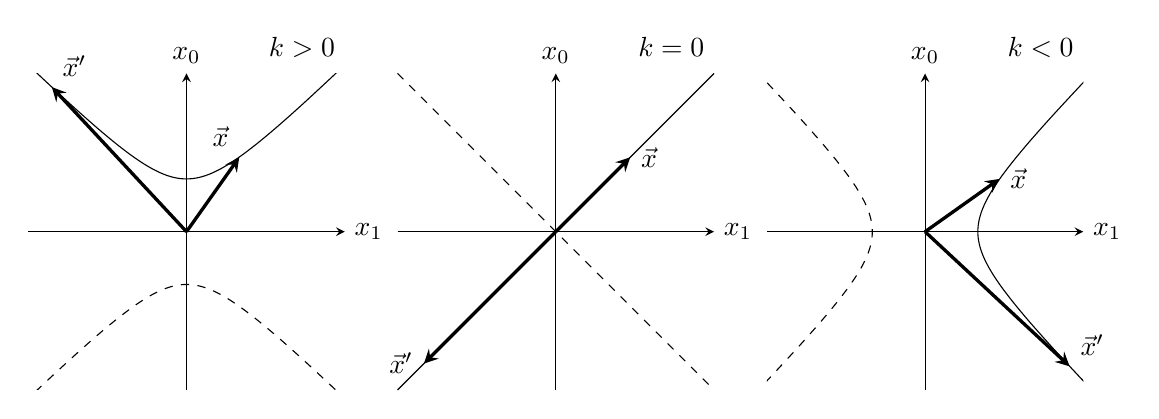
\begin{tikzpicture}[>=stealth, scale=0.67]
  \node[left] at (3, 3.5) {$k > 0$};
  \draw[->] (-3, 0) -- (3, 0) node[right] {$x_1$};
  \draw[->] (0, -3) -- (0, 3) node[above] {$x_0$};

  \draw[very thick,->] (0, 0) -- (1, 1.41) node[above left] {$\vec{x}$};
  \draw[very thick,->] (0, 0) -- (-2.552, 2.74) node[above right] {$\vec{x}'$};

  \begin{scope}
    \clip (-3, -3) rectangle (3, 3);
    \draw[domain=-1.4:1.4, smooth, variable=\t] plot ({tan(\t r)},{sec(\t r)});
    \draw[domain=-1.4:1.4, smooth, variable=\t, dashed] plot ({tan(\t r)},{-sec(\t r)});
  \end{scope}
\begin{scope}[xshift=7cm]
  \node[left] at (3, 3.5) {$k = 0$};
  \draw[->] (-3, 0) -- (3, 0) node[right] {$x_1$};
  \draw[->] (0, -3) -- (0, 3) node[above] {$x_0$};

  \draw[very thick,->] (0, 0) -- (1.41, 1.41) node[right] {$\vec{x}$};
  \draw[very thick,->] (0, 0) -- (-2.5, -2.5) node[left] {$\vec{x}'$};

  \draw (-3, -3) -- (3, 3);
  \draw[dashed] (-3, 3) -- (3, -3);
\end{scope}
\begin{scope}[xshift=14cm]
  \node[left] at (3, 3.5) {$k < 0$};
  \draw[->] (-3, 0) -- (3, 0) node[right] {$x_1$};
  \draw[->] (0, -3) -- (0, 3) node[above] {$x_0$};

  \draw[very thick,->] (0, 0) -- (1.41, 1) node[right] {$\vec{x}$};
  \draw[very thick,->] (0, 0) -- (2.74, -2.552) node[above right] {$\vec{x}'$};

  \begin{scope}
    \clip (-3, -3) rectangle (3, 3);
    \draw[domain=-1.4:1.4, smooth, variable=\t] plot ({sec(\t r)},{tan(\t r)});
    \draw[domain=-1.4:1.4, smooth, variable=\t, dashed] plot ({-sec(\t r)},{tan(\t r)});
  \end{scope}
\end{scope}
\end{tikzpicture}
\end{center}
For $k \neq 0$, we have a hyperbola, and for $k = 0$, we have a straight line.

Note that the dashed sections represent the other branch of the curve.
Since we required that $M_{0 0} > 0$, $\vec{x}$ and $\vec{x}'$ must both lie on the same branch.
\begin{remark}
  This is similar to how orthogonal transformations preserve the standard norm of vectors so vectors lying on a circle centered at the origin are mapped to another vector on the same circle.
  Instead, Lorentz transformations keep vectors on the same hyperbola branch instead of the same circle.
\end{remark}
\subsubsection{Application to Special Relativity}
We can rewrite:
\[
  M(\theta) =
  \frac{\sech \theta}{\sqrt{1 - \tanh^2 \theta}}
  \begin{pmatrix}
  \cosh \theta & \sinh \theta \\
  \sinh \theta  & \cosh \theta \\
  \end{pmatrix} =
  \frac{1}{\sqrt{1 - \tanh^2 \theta}} \begin{pmatrix}
  1 & \tanh \theta \\
  \tanh \theta & 1 \\
  \end{pmatrix}
\]
When working with special relativity use \textit{natural units}.
This means that we normalise the speed of light to be $c = 1$.
This means that all other velocities $v$ must be in the range $-1 < v < 1$.
We can then let $v = \tanh \theta$ for some $\theta$.

We then rename $x_0 \mapsto t$ to represent the \textit{time coordinate} and rename $x_1 \mapsto x$ to represent the \textit{space coordinate}.

The image of $\vec{x}$, $\vec{x}' = M\vec{x}$, then has components:
\[
  t' = \frac{1}{\sqrt{1 - v^2}}(t + vx) \text{ and } x' = \frac{1}{\sqrt{1 - v^2}}(x + vt)
\]

$x$ and $t$ represent a space and time coordinate in one spacetime reference frame and $x'$ and $t'$ are those but in some other reference frame with relative velocity $v$ to the initial frame.

This means that \textit{Lorentz transformations} relate the space and time coordinates for observers with relative velocity $v$, this is used heavily in \textit{Special Relativity} and is covered further in the course Dynamics and Relativity.

The factor $\gamma(v) = \frac{1}{\sqrt{1 - v^2}}$ is called the \textit{Lorentz factor} and gives rise to time dilation and length contraction effects.


Here we employed the active point of view by considering the transformation of vectors and saw that these transformations are moving the body, however, if we consider the passive point of view, then we can instead see the transformation as changing the reference frame whilst keeping the body fixed.
\subsubsection{Composition of Velocities}
We can use the product formula derived above to compose relativistic velocities:
\[
  M(\theta_1)M(\theta_2) = M(\underbrace{\theta_1 + \theta_2}_{\theta_3})
\]
If we set $v_i = \tanh(\theta_i)$ for $i = 1, 2, 3$, then:
\begin{align*}
  &\frac{1}{\sqrt{1 - v^{2}_{1}}\sqrt{1 - v^{2}_{2}}}
  \begin{pmatrix}
  1 & v_1 \\
  v_1 & 1 \\
  \end{pmatrix}
  \begin{pmatrix}
  1 & v_2 \\
  v_2 & 1 \\
  \end{pmatrix} =
  \frac{1}{\sqrt{1 - v^{2}_{3}}}
  \begin{pmatrix}
  1 & v_3 \\
  v_3 & 1 \\
  \end{pmatrix} \\
  \implies& \frac{1 + v_1 v_2}{\sqrt{1 - v^{2}_{1}}\sqrt{1 - v^{2}_{2}}} = \frac{1}{\sqrt{1 - v^{2}_{3}}} \text{ and }
  \frac{v_1 + v_2}{\sqrt{1 - v^{2}_{1}}\sqrt{1 - v^{2}_{2}}} = \frac{v_3}{\sqrt{1 - v^{2}_{3}}} \\
  \implies& v_3 = \frac{v_1 + v_2}{1 + v_1v_2}
\end{align*}
which is the composition of relativistic velocities in natural units (i.e. all $|v_i| < 1$).
\end{document}
